% ===== CHAPTER 9 =====
\chapter{微扰理论}
\label{chap:9}
\section{微扰理论}
\label{sec:9.1 Perturbation Theory}
    本章讨论第二种主要的量子力学近似方法——微扰理论。

    假设我们有一个系统,其定态哈密顿量为$\hat{H}$,我们无法通过求解薛定谔方程
    \begin{equation}
        \hat{H} \psi_n = E_n \psi_n
        \label{eq:9.1}
    \end{equation}
    来获得其束缚态本征函数和本征值。再假设:哈密顿量$\hat{H}$与某一满足以下我们可解的薛定谔方程系统的哈密顿量$\hat{H}^0$之间只存在微小的差异:
    \begin{equation}
        \hat{H}^0 \psi_n^{\left(0\right)} = E_n^{\left(0\right)} \psi_n^{\left(0\right)}
        \label{eq:9.2}
    \end{equation}
    一维非谐振子的哈密顿量就是一个例子:
    \begin{equation}
        \hat{H} = -\frac{\hbar^2}{2m} \frac{\mathrm{d}^2}{\mathrm{d}x^2} + \frac{1}{2}kx^2 + cx^3 + dx^4
        \label{eq:9.3}
    \end{equation}
    其哈密顿量(\ref{eq:9.3})与以下谐振子的哈密顿量十分接近:
    \begin{equation}
        \hat{H}^0 = -\frac{\hbar^2}{2m} \frac{\mathrm{d}^2}{\mathrm{d}x^2} + \frac{1}{2}kx^2
        \label{eq:9.4}
    \end{equation}
    若(\ref{eq:9.3})中的常数$c$和$d$很小,我们可以预测非谐振子的本征函数和本征值与谐振子的非常接近。

    我们称具有哈密顿量$\hat{H}^0$的系统为\textbf{未扰动系统}(unperturbed system),具有哈密顿量$\hat{H}$的系统为\textbf{扰动系统}(perturbed system)。二哈密顿量之间的不同$\hat{H}'$称为\textbf{微扰}(perturbation),记为:
    \begin{equation}
        \hat{H}' \equiv \hat{H} - \hat{H}^0
        \label{eq:9.5}
    \end{equation}
    \begin{equation}
        \boxed{
        \hat{H} = \hat{H}^0 + \hat{H}'
        }
        \label{eq:9.6}
    \end{equation}
    (符号$\prime$不表示微分。)对于具有哈密顿量(\ref{eq:9.3})的非谐振子,对相关的谐振子的微扰为$\hat{H}' = cx^3 + dx^4$。

    在$\hat{H}^0 \psi_n^{\left(0\right)} = E_n^{\left(0\right)} \psi_n^{\left(0\right)}$[式(\ref{eq:9.2})]中,$E_n^{\left(0\right)}$和$\psi_n^{\left(0\right)}$分别称为状态$n$的\textbf{未扰动能量}(unperturbed energy)和\textbf{未扰动波函数}(unperturbed wave function)。若$\hat{H}^0$为谐振子的哈密顿量(\ref{eq:9.4}),则$E_n^{\left(0\right)} = \left(n + \frac{1}{2}\right)h\nu$[式(\ref{eq:4.45})],其中的$n$是非负整数。(我们使用$n$代替$v$为了与微扰理论符号保持一致。)上标$^{(0)}$不表示基态。微扰理论可以应用于任何状态。下标$n$表示我们正在处理的状态。而上标$^{(0)}$表示未扰动系统的状态。

    我们的目标是将扰动系统位置的本征函数和本征值与未扰动系统已知的本征函数和本征值联系起来。为此,我们假定扰动是逐渐增加的,从未扰动系统到扰动系统的变化是连续的。在数学上,这相当于在哈密顿量中插入了一个参数$\lambda$,使得
    \begin{equation}
        \hat{H} = \hat{H}^0 + \lambda \hat{H}'
        \label{eq:9.7}
    \end{equation}
    当$\lambda$为零时,系统为未扰动系统。随着$\lambda$的增加,扰动逐渐变大,在$\lambda=1$时,扰动完全“被打开”。我们插入$\lambda$是为了将扰动本征函数和未扰动本征函数关联起来,最终设定$\lambda=1$并删去它。

    第9.1-9.7节处理定态哈密顿量和定态系统,第\ref{sec:9.8 Time-dependent Perturbation Theory}节处理含时微扰理论。

\section{非简并微扰理论}
\label{sec:9.2 Nondegenerate Perturbation Theory}
    微扰理论处理简并和非简并能级的方式不同。本节将研究微扰对非简并能级的影响。若某未扰动系统的能级是简并的,而另一些是非简并的,那么本节的处理方法将只适用于非简并能级。

\subsection*{非简并微扰理论}
    令$\psi_n^{\left(0\right)}$为能量为$E_n^{\left(0\right)}$的某个非简并未扰动系统的波函数。再令$\psi_n$为扰动系统的波函数,在施加扰动后,$\psi_n^{\left(0\right)}$变为$\psi_n$。由(\ref{eq:9.1})和(\ref{eq:9.7}),扰动态的薛定谔方程为
    \begin{equation}
        \hat{H}\psi_n = \left(\hat{H}^0 + \lambda \hat{H}'\right)\psi_n = E_n \psi_n
        \label{eq:9.8}
    \end{equation}
    由于(\ref{eq:9.8})中的哈密顿量与参数$\lambda$有关,本征函数$\psi_n$和本征值$E_n$也将与$\lambda$有关:
    \begin{equation*}
        \psi_n = \psi_n\left(\lambda, q\right), \quad E_n = E_n\left(\lambda\right)
    \end{equation*}
    其中$q$表示粒子的坐标。我们现在使用$\lambda$的Taylor级数(问题4.1)展开$\psi_n$和$E_n$:
    \begin{equation}
        \psi_n = \left. \psi_n \right|_{\lambda=0} + \left. \frac{\partial \psi_n}{\partial \lambda} \right|_{\lambda=0}\lambda + \left. \frac{\partial^2 \psi_n}{\partial \lambda^2} \right|_{\lambda=0}\frac{\lambda^2}{2!} + \cdots
        \label{eq:9.9}
    \end{equation}
    \begin{equation}
        E_n = \left. E_n \right|_{\lambda=0} + \left. \frac{\mathrm{d} E_n}{\mathrm{d} \lambda} \right|_{\lambda=0}\lambda + \left. \frac{\mathrm{d}^2 E_n}{\mathrm{d} \lambda^2} \right|_{\lambda=0}\frac{\lambda^2}{2!} + \cdots
        \label{eq:9.10}
    \end{equation}
    根据假设,当$\lambda \to 0$时,$\psi_n$和$E_n$分别趋近于$\psi_n^{\left(0\right)}$和$E_n^{\left(0\right)}$:
    \begin{equation}
        \left. \psi_n \right|_{\lambda=0} = \psi_n^{\left(0\right)}, \quad \left. E_n \right|_{\lambda=0} = E_n^{\left(0\right)}
        \label{eq:9.11}
    \end{equation}
    我们引入以下缩写:
    \begin{equation}
        \psi_n^{\left(k\right)} \equiv \frac{1}{k!} \left. \frac{\partial^k \psi_n}{\partial \lambda^k} \right|_{\lambda=0}, \quad E_n^{\left(k\right)} \equiv \frac{1}{k!} \left. \frac{\mathrm{d}^k E_n}{\mathrm{d} \lambda^k} \right|_{\lambda=0}, \quad k = 0, 1, 2, \ldots
        \label{eq:9.12}
    \end{equation}
    则(\ref{eq:9.9})和(\ref{eq:9.10})变为
    \begin{equation}
        \psi_n = \psi_n^{\left(0\right)} + \lambda \psi_n^{\left(1\right)} + \lambda^2 psi_n^{\left(2\right)} + \cdots + \lambda^k \psi_n^{\left(k\right)} + \cdots
        \label{eq:9.13}
    \end{equation}
    \begin{equation}
        E_n = E_n^{\left(0\right)} + \lambda E_n^{\left(1\right)} + \lambda^2 E_n^{\left(2\right)} + \cdots + \lambda^k E_n^{\left(k\right)} + \cdots
        \label{eq:9.14}
    \end{equation}
    对于$k = 1,2,3,\ldots$,我们称$\psi_n^{\left(k\right)}$和$E_n^{\left(k\right)}$分别为波函数和能量的\textbf{$k$级校正}($k$th-order correction)。我们假设级数(\ref{eq:9.13})和(\ref{eq:9.14})在$\lambda=1$处收敛,我们希望,对于小扰动,只取级数的前几项就能很好地逼近真实的能量和波函数。(通常,微扰理论的级数并不收敛,尽管如此,不收敛级数的前几项也能给出有用的近似值。)

    令$\psi_n^{\left(0\right)}$归一化:$\left\langle \psi_n^{\left(0\right)} \middle| \psi_n^{\left(0\right)} \right\rangle = 1$。与令$\psi_n$归一化不同,我们要求$\psi_n$满足
    \begin{equation}
        \left\langle \psi_n^{\left(0\right)} \middle| \psi_n \right\rangle = 1
        \label{eq:9.15}
    \end{equation}
    若$\psi_n$不满足该方程,则将常数$1/\left\langle \psi_n^{\left(0\right)} \middle| \psi_n \right\rangle$乘到$\psi_n$上,得到一个满足该性质的微扰波函数。条件(\ref{eq:9.15}),称为\textbf{中间归一化}(intermediate normalization),它简化了推导过程。注意:将$\psi_n$与一个常数相乘并不会改变薛定谔方程$\hat{H} \psi_n = E_n \psi_n$中的能量,所以应用中间归一化不会影响能量校正的结果。 如果需要,在计算结束时,可以将中间归一化的 $\psi_n$ 乘以一个常数,使其在通常意义上归一化。

    将(\ref{eq:9.13})带入$1 = \left\langle \psi_n^{\left(0\right)} \middle| \psi_n \right\rangle$[式(\ref{eq:9.15})],得到
    \begin{equation*}
        1 = \left\langle \psi_n^{\left(0\right)} \middle| \psi_n^{\left(0\right)} \right\rangle + \lambda \left\langle \psi_n^{\left(0\right)} \middle| \psi_n^{\left(1\right)} \right\rangle + \lambda^2 \left\langle \psi_n^{\left(0\right)} \middle| \psi_n^{\left(2\right)} \right\rangle + \cdots
    \end{equation*}
    由于该方程对介于$0$和$1$之间的任意$\lambda$都成立,如(\ref{eq:4.11})之后所证明的,方程两边 $\lambda$ 同次幂的系数必须相等。令$\lambda^0$的系数相等,我们有$1 = \left\langle \psi_n^{\left(0\right)} \middle| \psi_n^{\left(0\right)} \right\rangle$,由于$\psi_n^{\left(0\right)}$归一化,上式显然成立。令$\lambda^1$、$\lambda^2$等的系数相等,我们有
    \begin{equation}
        \left\langle \psi_n^{\left(0\right)} \middle| \psi_n^{\left(1\right)} \right\rangle = 0, \quad \left\langle \psi_n^{\left(0\right)} \middle| \psi_n^{\left(2\right)} \right\rangle = 0, \quad \text{etc.}
        \label{eq:9.16}
    \end{equation}
    使用中间归一化时,波函数的校正与 $\psi_n^{\left(0\right)}$ 正交。

    将(\ref{eq:9.13})和(\ref{eq:9.14})代入薛定谔方程(\ref{eq:9.8}),得到
    \begin{equation*}
        \begin{aligned}
            \left(\hat{H}^0 + \lambda\hat{H}'\right)&\left(\psi_n^{\left(0\right)} + \lambda\psi_n^{\left(1\right)} + \lambda^2\psi_n^{\left(2\right)}+\cdots\right) \\
            &= \left(E_n^{\left(0\right)} + \lambda E_n^{\left(1\right)} + \lambda^2 E_n^{\left(2\right)}+\cdots\right)\left(\psi_n^{\left(0\right)} + \lambda\psi_n^{\left(1\right)} + \lambda^2\psi_n^{\left(2\right)}+\cdots\right)
        \end{aligned}
    \end{equation*}
    将$\lambda$的同次幂进行归并,我们得到
    \begin{equation}
        \begin{aligned}
            \hat{H}^0 \psi_n^{\left(0\right)} &+ \lambda \left(\hat{H}'\psi_n^{\left(0\right)} + \hat{H}^0\psi_n^{\left(1\right)}\right) + \lambda^2 \left(\hat{H}^0\psi_n^{\left(2\right)} + \hat{H}'\psi_n^{\left(1\right)}\right) + \cdots \\
            &= E_n^{\left(0\right)} \psi_n^{\left(0\right)} + \lambda \left(E_n^{\left(1\right)} \psi_n^{\left(0\right)} + E_n^{\left(0\right)} \psi_n^{\left(1\right)}\right) + \lambda^2 \left(E_n^{\left(2\right)} \psi_n^{\left(0\right)} + E_n^{\left(1\right)} \psi_n^{\left(1\right)} + E_n^{\left(0\right)} \psi_n^{\left(2\right)}\right) + \cdots
        \end{aligned}
        \label{eq:9.17}
    \end{equation}
    现在(假设收敛性合适),要使 (\ref{eq:9.17}) 两边的两个级数对所有 $\lambda$ 值都相等,两个级数中 $\lambda$ 的同次幂的系数必须相等。

    令$\lambda^0$项的系数相等,我们得到$\hat{H}^0 \psi_n^{\left(0\right)} = E_n^{\left(0\right)} \psi_n^{\left(0\right)}$,这是未扰动系统的薛定谔方程(\ref{eq:9.2}),没有给我们有用的信息。

    令$\lambda^1$项的系数相等,我们得到
    \begin{equation*}
        \hat{H}'\psi_n^{\left(0\right)} + \hat{H}^0\psi_n^{\left(1\right)} = E_n^{\left(1\right)} \psi_n^{\left(0\right)} + E_n^{\left(0\right)} \psi_n^{\left(1\right)}
    \end{equation*}
    \begin{equation}
        \hat{H}^0\psi_n^{\left(1\right)} - E_n^{\left(0\right)} \psi_n^{\left(1\right)} = E_n^{\left(1\right)} \psi_n^{\left(0\right)} - \hat{H}'\psi_n^{\left(0\right)}
        \label{eq:9.18}
    \end{equation}

\subsection*{一级能量校正}

    为了求出$E_n^{\left(1\right)}$,我们将(\ref{eq:9.18})两边乘以$\psi_n^{\left(0\right)\ast}$并对全空间积分,有
    \begin{equation}
        \left\langle \psi_m^{\left(0\right)} \middle| \hat{H} \middle| \psi_n^{\left(1\right)} \right\rangle - E_n^{\left(0\right)} \left\langle \psi_m^{\left(0\right)} \middle| \psi_n^{\left(1\right)} \right\rangle = E_n^{\left(1\right)} \left\langle \psi_m^{\left(0\right)} \middle| \psi_n^{\left(0\right)} \right\rangle - \left\langle \psi_m^{\left(0\right)} \middle| \hat{H}' \middle| \psi_n^{\left(0\right)} \right\rangle
        \label{eq:9.19}
    \end{equation}
    其中用到了狄拉克符号[式(\ref{eq:7.1})和(\ref{eq:7.3})]。$\hat{H}^0$是厄米算符,使用厄米算符的性质(\ref{eq:7.12}),(\ref{eq:9.19})左侧的第一项变为
    \begin{equation}
        \begin{aligned}
            \left\langle \psi_m^{\left(0\right)} \middle| \hat{H}^0 \middle| \psi_n^{\left(1\right)} \right\rangle &= \left\langle \psi_m^{\left(1\right)} \middle| \hat{H}^0 \middle| \psi_n^{\left(0\right)} \right\rangle^{\ast} = \left\langle \psi_m^{\left(1\right)} \middle| \hat{H}^0 \psi_n^{\left(0\right)} \right\rangle^{\ast} \\
            &= \left\langle \psi_m^{\left(1\right)} \middle| E_n^{\left(m\right)} \psi_n^{\left(0\right)} \right\rangle^{\ast} = E_m^{\left(0\right)\ast} \left\langle \psi_n^{\left(1\right)} \middle| \psi_m^{\left(0\right)} \right\rangle^{\ast} = E_m^{\left(0\right)} \left\langle \psi_m^{\left(0\right)} \middle| \psi_n^{\left(1\right)} \right\rangle
        \end{aligned}
        \label{eq:9.20}
    \end{equation}
    其中我们用到了未扰动薛定谔方程$\hat{H}^0 \psi_m^{\left(0\right)} = E_m^{\left(0\right)} \psi_m^{\left(0\right)}$、$E_m^{\left(0\right)}$是实数以及(\ref{eq:7.4})。将(\ref{eq:9.20})代入(\ref{eq:9.19}),对未扰动本征函数使用正交方程$\left\langle \psi_m^{\left(0\right)} \middle| \psi_n^{\left(0\right)} \right\rangle = \delta_{mn}$,我们得到
    \begin{equation}
        \left(E_m^{\left(0\right)} - E_n^{\left(0\right)}\right)\left\langle \psi_m^{\left(0\right)} \middle| \psi_n^{\left(1\right)} \right\rangle = E_n^{\left(1\right)}\delta_{mn} - \left\langle \psi_m^{\left(0\right)} \middle| \hat{H}' \middle| \psi_n^{\left(0\right)} \right\rangle
        \label{eq:9.21}
    \end{equation}
    若$m=n$,则(\ref{eq:9.21})的左侧为零,(\ref{eq:9.21})变为
    \begin{equation}
        \boxed{
            E_n^{\left(1\right)} = \left\langle \psi_n^{\left(0\right)} \middle| \hat{H}' \middle| \psi_n^{\left(0\right)} \right\rangle = \int \psi_n^{\left(0\right)\ast} \hat{H}' \psi_n^{\left(0\right)} \:\mathrm{d}\tau
        }
        \label{eq:9.22}
    \end{equation}
    \textit{通过对作用于适当未扰动波函数的扰动 $\hat{H}'$ 求平均值,可以求出能量的一级校正。}

    在(\ref{eq:9.14})中令$\lambda=1$,我们得到
    \begin{equation}
        E_n \approx E_n^{\left(0\right)} + E_n^{\left(1\right)} = E_n^{\left(0\right)} + \int \psi_n^{\left(0\right)\ast} \hat{H}' \psi_n^{\left(0\right)} \:\mathrm{d}\tau
        \label{eq:9.23}
    \end{equation}

    \begin{examplebox}
        \textbf{例题:}对于具有哈密顿量(\ref{eq:9.3})的非谐振子,若未扰动系统取为谐振子,求基态的$E^{(1)}$。
        \\

        微扰由(\ref{eq:9.3})至(\ref{eq:9.5})给出:
        \begin{equation*}
            \hat{H}' = \hat{H} - \hat{H}^0 = cx^3 + dx^4
        \end{equation*}
        具有量子数为$v$状态的一级能量校正由(\ref{eq:9.22})给出:$E_v^{(1)} = \left\langle \psi_v^{(0)} \middle| cx^3 + dx^4 \middle| \psi_v^{(0)} \right\rangle$,其中$\psi_v^{(0)}$是状态$v$的谐振子波函数。对于$v=0$的基态,使用式$\psi_0^{\left(0\right)} = \left(\alpha /\pi\right)^{1/4} \mathrm{e}^{-\alpha x^2 / 2}$[式(\ref{eq:4.53})],有
        \begin{equation*}
            E_0^{\left(1\right)} = \left\langle \psi_0^{\left(0\right)} \middle| cx^3 + dx^4 \middle| \psi_0^{\left(0\right)} \right\rangle = \left(\frac{\alpha}{\pi}\right)^{1/2} \int_{-\infty}^{\infty} \mathrm{e}^{-\alpha x^2} \left(cx^3 + dx^4\right) \:\mathrm{d}x
        \end{equation*}
        从$-\infty$到$\infty$对奇函数$cx^3\mathrm{e}^{-\alpha x^2}$积分为零。使用附录(A.10)中的积分,令$n=2$;再对$\alpha$使用(\ref{eq:4.31}),得到
        \begin{equation*}
            E_0^{\left(1\right)} = 2d\left(\frac{\alpha}{\pi}\right)^{1/2} \int_{0}^{\infty} \mathrm{e}^{-\alpha x^2} x^4 \:\mathrm{d}x = \frac{3d}{4\alpha^2} = \frac{3dh^2}{64\pi^4 \nu^2 m^2}
        \end{equation*}
        未扰动基态能量为$E_0^{\left(0\right)} = \frac{1}{2}h\nu$,$E_0^{\left(0\right)} + E_0^{\left(1\right)} = \frac{1}{2}h\nu + \frac{3dh^2}{64\pi^4 \nu^2 m^2}$。
        \\

        \textbf{练习:}考虑一个单粒子一维系统,其势能函数满足
        \begin{equation*}
            V = \begin{cases}
                \infty, & x < 0 \\
                V = cx, & 0 \leq x < l \\
                \infty, & x \geq l
            \end{cases}
        \end{equation*}
        其中$c$是常数。

        (a)当$c>0$时,画出$V$的图象。

        (b)将该系统看作箱中粒子系统的微扰,求量子数为$n$状态的$E_n^{(1)}$。使用式 (\ref{eq:3.88}) 说明得到的答案是符合预期的。

        (\textit{部分答案:}(b)$\frac{1}{2}cl$。)
    \end{examplebox}

\subsection*{一级波函数校正}

    对于$m \neq n$,式(\ref{eq:9.21})为
    \begin{equation}
        \left(E_m^{\left(0\right)} - E_n^{\left(0\right)}\right)\left\langle \psi_m^{\left(0\right)} \middle| \psi_n^{\left(1\right)} \right\rangle = - \left\langle \psi_m^{\left(0\right)} \middle| \hat{H}' \middle| \psi_n^{\left(0\right)} \right\rangle, \quad m \neq n
        \label{eq:9.24}
    \end{equation}
    为了求出$\psi_n^{\left(1\right)}$,我们将其用厄米算符$\hat{H}^0$的未扰动本征函数$\psi_m^{\left(0\right)}$完整正交集展开:
    \begin{equation}
        \psi_n^{\left(1\right)} = \sum_{m} a_m \psi_m^{\left(0\right)}, \quad \text{其中} \quad a_m = \left\langle \psi_m^{\left(0\right)} \middle| \psi_n^{\left(1\right)} \right\rangle
        \label{eq:9.25}
    \end{equation}
    其中(\ref{eq:7.41})用于计算展开系数$a_m$。在(\ref{eq:9.24})中使用$a_m = \left\langle \psi_m^{\left(0\right)} \middle| \psi_n^{\left(1\right)} \right\rangle$,我们得到
    \begin{equation*}
        \left(E_m^{\left(0\right)} - E_n^{\left(0\right)}\right)a_m = - \left\langle \psi_m^{\left(0\right)} \middle| \hat{H}' \middle| \psi_n^{\left(0\right)} \right\rangle, \quad m \neq n
    \end{equation*}
    根据假设,能级$E_n^{\left(0\right)}$是非简并的,因此若$m \neq n$,有$E_m^{\left(0\right)} - E_n^{\left(0\right)} \neq 0$。两边同除以$\left(E_m^{\left(0\right)} - E_n^{\left(0\right)}\right)$,我们得到
    \begin{equation}
        a_m = \frac{\left\langle \psi_m^{\left(0\right)} \middle| \hat{H}' \middle| \psi_n^{\left(0\right)} \right\rangle}{E_n^{\left(0\right)} - E_m^{\left(0\right)}}, \quad m \neq n
        \label{eq:9.26}
    \end{equation}
    除了$\psi_n^{\left(0\right)}$的系数$a_n$外,$\psi_n^{\left(1\right)}$展开式(\ref{eq:9.25})的系数$a_m$都可以用(\ref{eq:9.26})求出。根据(\ref{eq:9.25})的第二个方程,$a_n = \left\langle \psi_n^{\left(0\right)} \middle| \psi_n^{\left(1\right)} \right\rangle$。回忆我们为$\psi_n$选择的中间归一化条件使得$\left\langle \psi_n^{\left(0\right)} \middle| \psi_n^{\left(1\right)} \right\rangle = 0$[式(\ref{eq:9.16})]。因此$a_n = \left\langle \psi_n^{\left(0\right)} \middle| \psi_n^{\left(1\right)} \right\rangle = 0$,方程(\ref{eq:9.25})和(\ref{eq:9.26})给出了波函数的一级校正:
    \begin{equation}
        \psi_n^{\left(1\right)} = \sum_{m \neq n} \frac{\left\langle \psi_m^{\left(0\right)} \middle| \hat{H}' \middle| \psi_n^{\left(0\right)} \right\rangle}{E_n^{\left(0\right)} - E_m^{\left(0\right)}} \psi_m^{\left(0\right)}
        \label{eq:9.27}
    \end{equation}
    符号$\sum_{m \neq n}$表示对所有未扰动的状态求和,除了状态$n$。

    在(\ref{eq:9.13})中令$\lambda=1$,仅使用波函数的一级校正,我们得到了微扰波函数的近似:
    \begin{equation}
        \psi_n \approx \psi_n^{\left(0\right)} + \sum_{m \neq n} \frac{\left\langle \psi_m^{\left(0\right)} \middle| \hat{H}' \middle| \psi_n^{\left(0\right)} \right\rangle}{E_n^{\left(0\right)} - E_m^{\left(0\right)}} \psi_m^{\left(0\right)}
        \label{eq:9.28}
    \end{equation}
    有关$\psi_n^{\left(2\right)}$及$\psi$的归一化,见\textit{Kemble}, Chapter XI。

\subsection*{二级能量校正}

    令$\lambda^2$项的系数相等,我们得到
    \begin{equation}
        \hat{H}^0\psi_n^{\left(2\right)} - E_n^{\left(0\right)} \psi_n^{\left(2\right)} = E_n^{\left(2\right)} \psi_n^{\left(0\right)} + E_n^{\left(1\right)} \psi_n^{\left(1\right)} - \hat{H}' \psi_n^{\left(1\right)}
        \label{eq:9.29}
    \end{equation}
    乘以$\psi_m^{\left(0\right)\ast}$并对全空间积分,我们得到
    \begin{equation}
        \begin{aligned}
            \left\langle \psi_m^{\left(0\right)} \middle| \hat{H}^0 \middle| \psi_n^{\left(2\right)} \right\rangle - E_n^{\left(0\right)}& \left\langle \psi_m^{\left(0\right)} \middle| \psi_n^{\left(2\right)} \right\rangle \\
            &= E_n^{\left(2\right)} \left\langle \psi_m^{\left(0\right)} \middle| \psi_n^{\left(0\right)} \right\rangle + E_n^{\left(1\right)} \left\langle \psi_m^{\left(0\right)} \middle| \psi_n^{\left(1\right)} \right\rangle - \left\langle \psi_m^{\left(0\right)} \middle| \hat{H}' \middle| \psi_n^{\left(1\right)} \right\rangle
        \end{aligned}
        \label{eq:9.30}
    \end{equation}
    该方程中的积分$\left\langle \psi_m^{\left(0\right)} \middle| \hat{H}^0 \middle| \psi_n^{\left(2\right)} \right\rangle$与(\ref{eq:9.20})中的积分相同,除了$\psi_n^{\left(2\right)}$代替了$\psi_n^{\left(1\right)}$。在(\ref{eq:9.20})中用$\psi_n^{\left(2\right)}$代替$\psi_n^{\left(1\right)}$,我们得到
    \begin{equation}
        \left\langle \psi_m^{\left(0\right)} \middle| \hat{H}^0 \middle| \psi_n^{\left(2\right)} \right\rangle = E_m^{\left(0\right)} \left\langle \psi_m^{\left(0\right)} \middle| \psi_n^{\left(2\right)} \right\rangle
        \label{eq:9.31}
    \end{equation}
    利用 (\ref{eq:9.31}) 和 (\ref{eq:9.30}) 中未扰动函数的正交性,可以得出
    \begin{equation}
        \left(E_m^{\left(0\right)} - E_n^{\left(0\right)}\right)\left\langle \psi_m^{\left(0\right)} \middle| \psi_n^{\left(2\right)} \right\rangle = E_n^{\left(2\right)} \delta_{mn} + E_n^{\left(1\right)} \left\langle \psi_m^{\left(0\right)} \middle| \psi_n^{\left(1\right)} \right\rangle - \left\langle \psi_m^{\left(0\right)} \middle| \hat{H}' \middle| \psi_n^{\left(1\right)} \right\rangle
        \label{eq:9.32}
    \end{equation}
    若$m=n$,则(\ref{eq:9.32})的左侧为零,得到
    \begin{equation*}
        E_n^{\left(2\right)} = - E_n^{\left(1\right)} \left\langle \psi_n^{\left(0\right)} \middle| \psi_n^{\left(1\right)} \right\rangle + \left\langle \psi_n^{\left(0\right)} \middle| \hat{H}' \middle| \psi_n^{\left(1\right)} \right\rangle 
    \end{equation*}
    \begin{equation}
        E_n^{\left(2\right)} = \left\langle \psi_n^{\left(0\right)} \middle| \hat{H}' \middle| \psi_n^{\left(1\right)} \right\rangle
        \label{eq:9.33}
    \end{equation}
    因为$\left\langle \psi_n^{\left(0\right)} \middle| \psi_n^{\left(1\right)} \right\rangle = 0$[式(\ref{eq:9.16})]。从(\ref{eq:9.33})可知,要找到能量的\textit{二}级校正,我们只需要直到波函数的\textit{一}级校正。事实上,可以证明:知道$\psi_n^{\left(1\right)}$也足以确定$E_n^{\left(3\right)}$。

    一般地,可以证明:\textit{若我们知道波函数的$k$级校正,则可以确定能量的$2k+1$级校正。}(见\textit{Bates}, Vol. I, p. 184。)

    将(\ref{eq:9.27})中的$\psi_n^{\left(1\right)}$代入(\ref{eq:9.33}),我们得到
    \begin{equation}
        E_n^{\left(2\right)} = \sum_{m \neq n} \frac{\left\langle \psi_m^{\left(0\right)} \middle| \hat{H}' \middle| \psi_n^{\left(0\right)} \right\rangle}{E_n^{\left(0\right)} - E_m^{\left(0\right)}} \left\langle \psi_n^{\left(0\right)} \middle| \hat{H}' \middle| \psi_m^{\left(0\right)} \right\rangle
        \label{eq:9.34}
    \end{equation}
    由于展开系数$a_m$[式(\ref{eq:9.26})]是常数,可以提到积分外面。由于$\hat{H}'$是厄米算符,我们有
    \begin{equation*}
        \begin{aligned}
            \left\langle \psi_m^{\left(0\right)} \middle| \hat{H}' \middle| \psi_n^{\left(0\right)} \right\rangle \left\langle \psi_n^{\left(0\right)} \middle| \hat{H}' \middle| \psi_m^{\left(0\right)} \right\rangle &= \left\langle \psi_m^{\left(0\right)} \middle| \hat{H}' \middle| \psi_n^{\left(0\right)} \right\rangle \left\langle \psi_m^{\left(0\right)} \middle| \hat{H}' \middle| \psi_n^{\left(0\right)} \right\rangle^{\ast} \\
            &= \left|\left\langle \psi_m^{\left(0\right)} \middle| \hat{H}' \middle| \psi_n^{\left(0\right)} \right\rangle\right|^2
        \end{aligned}
    \end{equation*}
    则(\ref{eq:9.34})变为
    \begin{equation}
        E_n^{\left(2\right)} = \sum_{m \neq n} \frac{\left|\left\langle \psi_m^{\left(0\right)} \middle| \hat{H}' \middle| \psi_n^{\left(0\right)} \right\rangle\right|^2}{E_n^{\left(0\right)} - E_m^{\left(0\right)}}
        \label{eq:9.35}
    \end{equation}
    这正是我们需要的,用未扰动波函数和能量表示的$E_n^{\left(2\right)}$。

    将$E_n^{\left(2\right)}$和$\lambda=1$代入(\ref{eq:9.14}),可以得到微扰态能量的近似值为
    \begin{equation}
        E_n \approx E_n^{\left(0\right)} + H'_{nn} + \sum_{m \neq n} \frac{\left|\left\langle \psi_m^{\left(0\right)} \middle| \hat{H}' \middle| \psi_n^{\left(0\right)} \right\rangle\right|^2}{E_n^{\left(0\right)} - E_m^{\left(0\right)}}
        \label{eq:9.36}
    \end{equation}
    其中的积分是对未扰动归一化波函数的积分。

    有关高阶能量修正的公式,请参见\textit{Bates},Volume I,pages 181-185 。本节提出的微扰理论形式称为\textit{瑞利-薛定谔微扰理论}(Rayleigh-Schrödinger perturbation theory);还存在其他方法。

\subsection*{讨论}

    方程(\ref{eq:9.28})表明:作用在波函数$\psi_n^{\left(0\right)}$上的的微扰相当于“掺和”进了其他状态$\psi_m^{\left(0\right)},\:m \neq n$的贡献。由于因子$1/\left(E_n^{\left(0\right)} - E_m^{\left(0\right)}\right)$,对微扰波函数最重要的贡献来源于(除了$\psi_n^{\left(0\right)}$之外)能量最接近$n$的状态。

    要计算能量的一级校正,我们必须只计算单积分 $H'_{nn}$,而要计算能量的二级校正,我们必须计算第 $n$ 个状态和所有其他状态 $m$ 之间的 $\hat{H}'$ 矩阵元素,然后执行 (\ref{eq:9.35}) 中的无限求和。在很多情况下,二级校正难以准确计算。处理三级和更高的就更难了。

    (\ref{eq:9.28}) 和 (\ref{eq:9.36}) 中的和是不同状态的和,而不是不同能量值的和。如果某些能级(第 $n$ 个能级除外)是简并的,我们必须在总和中为简并能级对应的每个线性无关波函数加入某个项。

    我们在 (\ref{eq:9.28}) 和 (\ref{eq:9.36}) 中对状态求和,是因为我们需要一组完整的函数来展开 (\ref{eq:9.25}) ,因此我们必须在求和中包含所有线性无关的波函数。如果未扰动问题具有连续的波函数(例如氢原子),我们还必须对连续波函数进行积分,这样才能得到一组完整的波函数。若$\psi_E^{\left(0\right)}$是能量为$E$的未扰动连续波函数,则(\ref{eq:9.27})和(\ref{eq:9.35})变为
    \begin{equation*}
        \psi_n^{\left(1\right)} = \sum_{m \neq n} \frac{H'_{nn}}{E_n^{\left(0\right)} - E_m^{\left(0\right)}} \psi_m^{\left(0\right)} + \int \frac{H'_{E,n}}{E_n^{\left(0\right)} - E^{\left(0\right)}} \psi_E^{\left(0\right)} \:\mathrm{d}E^{\left(0\right)}
    \end{equation*}
    \begin{equation}
        E_n^{\left(2\right)} = \sum_{m \neq n} \frac{\left|H'_{mn}\right|^2}{E_n^{\left(0\right)} - E_m^{\left(0\right)}} + \int \frac{\left|H'_{E,n}\right|^2}{E_n^{\left(0\right)} - E^{\left(0\right)}} \:\mathrm{d}E^{\left(0\right)}
        \label{eq:9.37}
    \end{equation}
    其中$H'_{E,n} = \left\langle \psi_E^{\left(0\right)} \middle| \hat{H}' \middle| \psi_n^{\left(0\right)} \right\rangle$。这些方程中的积分是在连续态能量范围内进行的(例如,氢原子的能量从零到无穷大)。未扰动问题中连续态的存在使得 $E_n^{\left(2\right)}$ 的计算变得更加困难。

\subsection*{变分法和微扰法的比较}

    微扰法适用于系统的所有束缚态。虽然第 \ref{sec:8.1 The Variation Theorem} 节所述的变分原理只适用于给定对称性的最低态,但我们可以用线性变分法来处理束缚激发态。

    由于需要计算二级和高级能量校正中出现的离散态的无限和以及连续态的积分,微扰计算通常很难进行。

    在微扰法中,能量的计算($2k+1$ 级)比波函数的计算($k$ 级)要精确得多。在变分法中也存在同样的情况,我们可以用一个相当不准确的波函数得到一个相当好的能量。如果计算能量以外的其他性质,结果通常不如计算出的能量可靠。

\subsection*{变分-微扰法}

    通过变分-微扰法,我们可以精确地估算出系统基态的 $E^{\left(2\right)}$ 和高级扰动理论能量校正,而无需计算 (\ref{eq:9.36}) 中的无限和。该方法基于以下不等式:
    \begin{equation}
        \left\langle u \middle| \hat{H}^0 - E_g^{\left(0\right)} \middle| u \right\rangle + \left\langle u \middle| \hat{H}' - E_g^{\left(1\right)} \middle| \psi_g^{\left(0\right)} \right\rangle + \left\langle \psi_g^{\left(0\right)} \middle| \hat{H}' - E_g^{\left(1\right)} \middle| u \right\rangle \geq E_g^{\left(2\right)}
        \label{eq:9.38}
    \end{equation}
    其中$u$是任意满足定解条件的品优函数,下标$g$表示基态。(\ref{eq:9.38})的证明,参见\textit{Hameka}, Section 7-9。把 $u$ 看作一个试探函数,我们改变参数,使 (\ref{eq:9.38}) 左侧最小化,就可以估算出$E_g^{\left(2\right)}$。函数$u$原来就是$\psi_g^{\left(1\right)}$的近似——基态波函数的一级校正,$u$还可以用来估算$E_g^{\left(3\right)}$。类似的变分法可用于找到对基态能量和波函数的高级校正。

\section{微扰理论求解基态氦原子}
\label{sec:9.3 Perturbation Treatment of the Helium-Atom Ground State}
    氦原子有两个电子,其原子核带$+2\mathrm{e}$的电荷。我们将认为原子核处于静止状态(第 \ref{sec:6.6 The Bound-State Hydrogen-Atom Wave Functions} 节),并将坐标系的原点放在原子核上。电子1和2的坐标分别为$\left(x_1,y_1,z_1\right)$和$\left(x_2,y_2,z_2\right)$;见图\ref{fig:9.1}。
    \begin{figure}[ht]
        \centering
        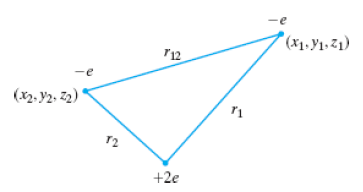
\includegraphics[width=0.5\textwidth]{Figures/9.1.png}
        \caption{氦原子中的粒子间距。}
        \label{fig:9.1}
    \end{figure}

    如果我们把核电荷数记为$+Z\mathrm{e}$而不是$+2\mathrm{e}$,就能处理类氦离子\ce{H^-}、\ce{Li^+}和\ce{Be^2+}。哈密顿算符为
    \begin{equation}
        \hat{H} = -\frac{\hbar^2}{2m_{\mathrm{e}}}\nabla_1^2 - \frac{\hbar^2}{2m_{\mathrm{e}}}\nabla_2^2 - \frac{Z\mathrm{e}^2}{4\pi\varepsilon_0r_1} - \frac{Z\mathrm{e}^2}{4\pi\varepsilon_0r_2} + \frac{\mathrm{e}^2}{4\pi\varepsilon_0r_{12}}
        \label{eq:9.39}
    \end{equation}
    其中$m_{\mathrm{e}}$是电子的质量,$r_1$和$r_2$分别是电子1和电子2到原子核的距离,$r_{12}$是两个电子之间的距离。前两项为电子动能的算符[式(\ref{eq:3.48})]。第三项和第四项是电子与原子核之间的吸引势。最后一项是电子间的排斥势[式(\ref{eq:6.58})]。请注意,相互作用粒子系统的势能不能写成单个粒子的势能之和。势能是整个系统的属性。

    薛定谔方程涉及六个独立变量,每个电子有三个坐标。在球坐标系中,$\psi = \psi\left(r_1,\theta_1,\phi_1,r_2,\theta_2,\phi_2\right)$。

    算符$\nabla_1^2$由将(\ref{eq:6.6})中的$r,\theta,\phi$替换为$r_1,\theta_1,\phi_1$给出。变量$r_{12}$为$r_{12} = \left[\left(x_1 - x_2\right)^2 + \left(y_1 - y_2\right)^2\right.$\\$\left. + \left(z_1 - z_2\right)^2\right]^{1/2}$,使用球坐标系和直角坐标系之间的关系,我们可以用$r_1,r_2,\theta_1,\theta_2,\phi_1,\phi_2$来表示$r_{12}$。

    由于$\mathrm{e}^2 / 4\pi \varepsilon_0r_{12}$项的存在,氦原子的薛定谔方程在任何坐标系中都无法分离变量,因此我们必须使用近似方法。微扰法将哈密顿算符(\ref{eq:9.39})分为两个部分,$\hat{H}^0$和$\hat{H}'$,其中$\hat{H}^0$是一个可精确求解系统的哈密顿算符。若我们选择s
    \begin{equation}
        \hat{H}^0 = -\frac{\hbar^2}{2m_{\mathrm{e}}}\nabla_1^2 - \frac{Z\mathrm{e}^2}{4\pi\varepsilon_0r_1} - \frac{\hbar^2}{2m_{\mathrm{e}}}\nabla_2^2 - \frac{Z\mathrm{e}^2}{4\pi\varepsilon_0r_2}
        \label{eq:9.40}
    \end{equation}
    \begin{equation}
        \hat{H}' = \frac{\mathrm{e}^2}{4\pi\varepsilon_0r_{12}}
        \label{eq:9.41}
    \end{equation}
    那么$\hat{H}^0$是两个类氢哈密顿算符的加和,每个算符各有一个电子:
    \begin{equation}
        \hat{H}^0 = \hat{H}_1^0 + \hat{H}_2^0
        \label{eq:9.42}
    \end{equation}
    \begin{equation}
        \hat{H}_1^0 \equiv -\frac{\hbar^2}{2m_{\mathrm{e}}}\nabla_1^2 - \frac{Z\mathrm{e}^2}{4\pi\varepsilon_0r_1}, \quad \hat{H}_2^0 \equiv -\frac{\hbar^2}{2m_{\mathrm{e}}}\nabla_2^2 - \frac{Z\mathrm{e}^2}{4\pi\varepsilon_0r_2}
        \label{eq:9.43}
    \end{equation}
    未受扰动的系统是两个电子互不施力的氦原子。虽然这样的系统并不存在,但这并不妨碍我们将微扰理论应用于这一系统。

    由于未扰动哈密顿算符(\ref{eq:9.42})是两个独立粒子的哈密顿算符之和,我们可以利用公式 (\ref{eq:6.18}) 至 (\ref{eq:6.24}) 的变量分离结果得出结论:未扰动波函数的形式为
    \begin{equation}
        \psi^{\left(0\right)}\left(r_1,\theta_1,\phi_1,r_2,\theta_2,\phi_2\right) = F_1\left(r_1,\theta_1,\phi_1\right) F_2\left(r_2,\theta_2,\phi_2\right)
        \label{eq:9.44}
    \end{equation}
    未扰动能量为
    \begin{equation}
        E^{\left(0\right)} = E_1 + E_2
        \label{eq:9.45}
    \end{equation}
    \begin{equation}
        \hat{H}_1^0 F_1 = E_1 F_1, \quad \hat{H}_2^0 F_2 = E_2 F_2
        \label{eq:9.46}
    \end{equation}
    由于$\hat{H}_1^0$和$\hat{H}_2^0$是类氢哈密顿算符,(\ref{eq:9.46})的解为类氢本征函数和本征值。根据(\ref{eq:6.94}),我们有
    \begin{equation}
        E_1 = -\frac{Z^2}{n_1^2}\frac{m_{\mathrm{e}}e^4}{8\pi^2\varepsilon_0a_0}, \quad E_2 = -\frac{Z^2}{n_2^2}\frac{m_{\mathrm{e}}e^4}{8\pi^2\varepsilon_0a_0}
        \label{eq:9.47}
    \end{equation}
    \begin{equation}
        E^{\left(0\right)} = -Z^2\left(\frac{1}{n_1^2} + \frac{1}{n_2^2}\right)\frac{\mathrm{e}^2}{8\pi\varepsilon_0a_0}, \quad \begin{aligned}
            n_1 = & 1, 2, 3, \ldots \\
            n_2 = & 1, 2, 3, \ldots
        \end{aligned}
        \label{eq:9.48}
    \end{equation}
    其中$a_0$是玻尔半径。公式 (\ref{eq:9.48}) 给出了两个电子都与原子核结合的状态的零级能量。\ce{He} 原子也有连续态。

    最低能级满足$n_1 = 1,\: n_2 = 1$,其零级波函数[式(\ref{eq:6.104})]为
    \begin{equation}
        \psi_{1s^2}^{\left(0\right)} = \frac{1}{\pi^{1/2}}\left(\frac{Z}{a_0}\right)^{3/2} \mathrm{e}^{-Zr_1/a_0} \cdot \frac{1}{\pi^{1/2}}\left(\frac{Z}{a_0}\right)^{3/2} \mathrm{e}^{-Zr_2/a_0} = 1s\left(1\right)1s\left(2\right)
        \label{eq:9.49}
    \end{equation}
    其中$1s\left(1\right)1s\left(2\right)$表示电子1和2的类氢$1s$波函数的乘积,下标表示两个电子都在类氢$1s$轨道中。(请注意,将电子分配到轨道并将原子波函数写成单电子轨道函数的乘积的过程只是一种\textit{近似}。)该未扰动基态能量为
    \begin{equation}
        E^{\left(0\right)}_{1s^2} = -Z^2\left(2\right)\frac{\mathrm{e}^2}{8\pi\varepsilon_0a_0}
        \label{eq:9.50}
    \end{equation}
    $-\mathrm{e}^2 / 8\pi\varepsilon_0a_0$是氢原子的基态能量(假设原子核无限重)等于$213.606 \: \mathrm{eV}$[式(\ref{eq:6.105})-(\ref{eq:6.108})]。若$a_0$中电子的质量$m_{\mathrm{e}}$被替换为\ce{He}原子的折合质量,则$-\mathrm{e}^2 / 8\pi\varepsilon_0a_0$的值变为$-13.604 \: \mathrm{eV}$,我们将用这个数字来(部分地)校正 \ce{He} 中的核运动。对于氦原子,$Z=2$,(\ref{eq:9.50})为$-8\left(13.604 \: \mathrm{eV}\right) = -108.83 \: \mathrm{eV}$:
    \begin{equation}
        E^{\left(0\right)}_{1s^2} = -108.83 \: \mathrm{eV}
        \label{eq:9.51}
    \end{equation}

    这个零级能量与真正的氦原子基态能量相比如何?\ce{He}原子第一电离能的实验值为$24.587 \: \mathrm{eV}$。\ce{He} 的第二电离能很容易从理论上计算出来,因为它是类氢离子\ce{He^+}的电离能,等于$2^2\left(13.604 \: \mathrm{eV}\right) = 54.416 \: \mathrm{eV}$。如果我们选择完全电离原子的能量为零[这一选择隐含在 (\ref{eq:9.39}) 中],那么氦原子的基态能量为$-\left(24.587 + 54.416\right) \: \mathrm{eV} = -79.00 \: \mathrm{eV}$。零级能量 (\ref{eq:9.51}) 的误差为 $38\%$。我们本应预料到如此大的误差,因为微扰项$\mathrm{e}^2 / 4\pi\varepsilon_0r_{12}$并不小。

    下一步是计算能量的一级微扰校正。未扰动基态是非简并的,使用(\ref{eq:9.22})和(\ref{eq:9.49}),得到
    \begin{equation*}
        E^{\left(1\right)} = \left\langle \psi^{\left(0\right)} \middle| \hat{H}' \middle| \psi^{\left(0\right)} \right\rangle
    \end{equation*}
    \begin{equation}
        \begin{aligned}
            E^{\left(1\right)} = \frac{Z^6\mathrm{e}^2}{\left(4\pi\varepsilon_0\right)\pi^2a_0^6} \int_{0}^{2\pi} \int_{0}^{2\pi} \int_{0}^{\pi} \int_{0}^{\pi} \int_{0}^{\infty} & \int_{0}^{\infty}  \mathrm{e}^{-2Zr_1/a_0} \mathrm{e}^{-2Zr_2/a_0} \frac{1}{r_{12}}r_1^2 \sin\theta_1 \\
            & \times r^2 _2 \sin\theta_2 \:\mathrm{d}r_1 \:\mathrm{d}r_2 \:\mathrm{d}\theta_1 \:\mathrm{d}\theta_2 \:\mathrm{d}\phi_1 \:\mathrm{d}\phi_2
        \end{aligned}
        \label{eq:9.52}
    \end{equation}
    这个双电子问题的体积微元包含两个电子的坐标;$\mathrm{d}\tau \equiv \mathrm{d}\tau_1 \mathrm{d}\tau_2$。(\ref{eq:9.52})中的积分可以用球谐函数对$1/r_{12}$进行展开来计算,如问题9.14所述。可以发现,
    \begin{equation}
        E^{\left(1\right)} = \frac{5Z}{8}\left(\frac{\mathrm{e}^2}{4\pi\varepsilon_0a_0}\right)
        \label{eq:9.53}
    \end{equation}
    回忆一下,当我们使用\ce{He}的折合质量时,$\frac{1}{2}\mathrm{e}^2/4\pi\varepsilon_0a_0$的值为$13.604 \: \mathrm{eV}$,再令$Z=2$,我们得到了氦原子基态能量的一级校正:
    \begin{equation*}
        E^{\left(1\right)} = \frac{10}{4}\left(13.604 \: \mathrm{eV}\right) = 34.01 \: \mathrm{eV}
    \end{equation*}

    现在能量的近似值为
    \begin{equation}
        E^{\left(0\right)} + E^{\left(1\right)} = -108.83 \: \mathrm{eV} + 34.01 \: \mathrm{eV} = -74.82 \: \mathrm{eV}
        \label{eq:9.54}
    \end{equation}
    与实验值$-79.00 \: \mathrm{eV}$相比,误差为$5.3\%$。

    要计算对波函数的一级校正和对能量的高级校正,需要计算未扰动的基态和所有激发态(包括连续态)之间的 $1/r_{12}$ 矩阵元素,并进行适当的求和与积分。目前还没有人知道如何直接计算 $E^{\left(1\right)}$ 的所有贡献。请注意,$\psi^{\left(1\right)}$ 的作用是将 $1s^2$ 以外其他构型的贡献混入波函数。对氦的真实基态波函数贡献最大的是 $1s^2$ 构型,即未扰动(零阶)波函数。

    氦原子基态的$E^{\left(2\right)}$值已使用变分-微扰法(\ref{eq:9.38})得到计算结果。Scherr和Knight使用 100 项的试探函数,得到了六级波函数校正极其精确的近似值,从而得到了十三级能量校正的近似值[C. W. Scherr and R. E. Knight, \textit{Rev. Mod. Phys.}, \textbf{35}, 436 (1963)]。有关计算401级能量校正,见J. D. Baker et al., \textit{Phys. Rev. A}, \textbf{41}, 1247 (1990)。二级校正$E^{\left(2\right)}$的值为$-4.29 \: \mathrm{eV}$,$E^{\left(3\right)}$为$+0.12 \: \mathrm{eV}$。根据三级校正,我们得到基态能量为
    \begin{equation*}
        E \approx -108.83 \: \mathrm{eV} + 34.01 \: \mathrm{eV} - 4.29 \: \mathrm{eV} + 0.12 \: \mathrm{eV} = -78.99 \: \mathrm{eV}
    \end{equation*}
    与实验值$-79.00 \: \mathrm{eV}$很接近了。通过引入十三级校正,Scherr和Knight得到了基态氦原子能量为$-2.90372433 \left(\mathrm{e}^2 / 4\pi\varepsilon_0a_0\right)$,与将在下一节讲述的纯变分计算获得的结果$-2.90372438 \left(\mathrm{e}^2 / 4\pi\varepsilon_0a_0\right)$非常接近。

    可以证明氦原子能量的微扰理论级数展开是收敛的。见[R. Ahlrichs, \textit{Phys. Rev. A}, \textbf{5}, 605 (1972)]。

    \begin{quote}
        \small
        \noindent 我们无法找到双电子基态 \ce{He} 原子的精确波函数和能量,但值得注意的是,我们已经找到了双电子问题的薛定谔方程的基态精确解。这是一个假想原子[称为\textit{胡克定律原子或谐波原子}(Hooke's-law atom or harmonium)],其哈密顿算符为
        \begin{equation*}
            \hat{H} = -\frac{\hbar^2}{2m_{\mathrm{e}}}\nabla_1^2 - \frac{\hbar^2}{2m_{\mathrm{e}}}\nabla_2^2 + \frac{1}{2}k\left(r_1^2 + r_2^2\right) + \frac{\mathrm{e}^2}{4\pi\varepsilon_0r_{12}}
        \end{equation*}
        其中$r_1$和$r_2$是电子到原点的距离。对于力常数$k$的特定值,可以精确解得基态波函数和能量。见\url{en.wikipedia.org/wiki/Hooke’s_atom}。
    \end{quote}

\section{变分法求解基态氦}
\label{sec:9.4 Variational Treatments of the Ground State of Helium}
    在上节中,我们将氦原子的哈密顿算符写作$\hat{H} = \hat{H}^0 + \hat{H}'$,其中$\hat{H}^0$的基态本征函数$\psi_g^{\left(0\right)}$由(\ref{eq:9.49})给出。若我们在变分积分中,用零级微扰理论基态波函数$\psi_g^{\left(0\right)}$作为变分函数$\phi$会发生什么呢?变分积分$\left\langle \phi \middle| \hat{H} \middle| \phi \right\rangle = \left\langle \phi \middle| \hat{H} \phi \right\rangle$将变为
    \begin{equation}
        \begin{aligned}
            \left\langle \phi \middle| \hat{H} \middle| \phi \right\rangle &= \left\langle \psi_g^{\left(0\right)} \middle| \hat{H}^0 + \hat{H}' \middle| \psi_g^{\left(0\right)} \right\rangle = \left\langle \psi_g^{\left(0\right)} \middle| \hat{H}^0\psi_g^{\left(0\right)} + \hat{H}' \psi_g^{\left(0\right)} \right\rangle \\
            &= \left\langle \psi_g^{\left(0\right)} \middle| E_g^{\left(0\right)}\psi_g^{\left(0\right)} \right\rangle + \left\langle \psi_g^{\left(0\right)} \middle| \hat{H}' \psi_g^{\left(0\right)} \right\rangle = E_g^{\left(0\right)} + E_g^{\left(1\right)}
        \end{aligned}
        \label{eq:9.55}
    \end{equation}
    因为$\hat{H}\psi_g^{\left(0\right)} = E_g^{\left(0\right)}\psi_g^{\left(0\right)}$、$\left\langle \psi_g^{\left(0\right)} \middle| \psi_g^{\left(0\right)} \right\rangle = 1$,以及$E_g^{\left(1\right)} = \left\langle \psi_g^{\left(0\right)} \middle| \hat{H}' \middle| \psi_g^{\left(0\right)} \right\rangle$[式(\ref{eq:9.22})]。使用$\psi_g^{\left(0\right)}$作为变分函数得到了与一级变分理论相同的结果。

    现在,考虑氦原子基态的变分函数。如果我们使用$\psi_n^{\left(0\right)}$[式(\ref{eq:9.49})]作为试探函数,会得到一级微扰结果$-74.82 \: \mathrm{eV}$。为了改进这一结果,我们在(\ref{eq:9.49})中引入一个变分参数。我们尝试归一化函数
    \begin{equation}
        \phi = \frac{1}{\pi} \left(\frac{\zeta}{a_0}\right)^3 \mathrm{e}^{-\zeta r_1/a_0} \mathrm{e}^{-\zeta r_2/a_0}
        \label{eq:9.56}
    \end{equation}
    该函数通过将(\ref{eq:9.49})中真实核电荷数$Z$替换为试探参数$\zeta$(Zeta)而得。$\zeta$有一个简单的物理解释。由于一个电子往往会将另一个电子屏蔽在原子核之外,因此每个电子所带的有效核电荷略小于全核电荷 $Z$。如果一个电子将另一个电子完全屏蔽在原子核之外,我们就会得到 $Z-1$ 的有效核电荷。由于两个电子位于同一轨道,它们只能部分地相互屏蔽。因此,我们希望$\zeta$介于 $Z-1$ 和 $Z$ 之间。

    现在我们来计算变分积分。为了方便起见,我们将氦哈密顿算符(\ref{eq:9.39})重写为
    \begin{equation}
        \hat{H} = \left[-\frac{\hbar^2}{2m_{\mathrm{e}}}\nabla_1^2 - \frac{\zeta\mathrm{e}^2}{4\pi\varepsilon_0r_1} - \frac{\hbar^2}{2m_{\mathrm{e}}}\nabla_2^2 - \frac{\zeta\mathrm{e}^2}{4\pi\varepsilon_0r_2} \right] + \left(\zeta - Z\right)\frac{e^2}{4\pi\varepsilon_0r_{1}} + \left(\zeta - Z\right)\frac{e^2}{4\pi\varepsilon_0r_{2}} + \frac{\mathrm{e}^2}{4\pi\varepsilon_0r_{12}}
        \label{eq:9.57}
    \end{equation}
    其中涉及 $\zeta$ 的项被相加和相减。(\ref{eq:9.57}) 中括号内的项是有效核电荷 $\zeta$ 的两个类氢哈密顿量的总和。此外,试探函数 (\ref{eq:9.56}) 是核电荷 $\zeta$ 的两个类氢 $1s$ 函数的乘积。因此,当这些项作用于 $\phi$ 时,我们就得到了一个本征方程,本征值是核电荷 $\zeta$ 的两个类氢 $1s$ 的能量之和:
    \begin{equation}
        \left[-\frac{\hbar^2}{2m_{\mathrm{e}}}\nabla_1^2 - \frac{\zeta\mathrm{e}^2}{4\pi\varepsilon_0r_1} - \frac{\hbar^2}{2m_{\mathrm{e}}}\nabla_2^2 - \frac{\zeta\mathrm{e}^2}{4\pi\varepsilon_0r_2} \right] \phi = -\zeta^2\left(2\right)\frac{\mathrm{e}^2}{8\pi\varepsilon_0a_0}\phi
        \label{eq:9.58}
    \end{equation}
    使用(\ref{eq:9.57})和(\ref{eq:9.58}),我们可以计算变分积分
    \begin{equation}
        \begin{aligned}
            \int \phi^* \hat{H} \phi \:\mathrm{d}\tau = &-\zeta^2\frac{\mathrm{e}^2}{4\pi\varepsilon_0a_0} \int \phi^* \phi \:\mathrm{d}\tau + \frac{\left(\zeta - Z\right)\mathrm{e}^2}{4\pi\varepsilon_0} \int \frac{\phi^*\phi}{r_1} \:\mathrm{d}\tau \\
            &+ \frac{\left(\zeta - Z\right)\mathrm{e}^2}{4\pi\varepsilon_0} \int \frac{\phi^*\phi}{r_2} \:\mathrm{d}\tau + \frac{\mathrm{e}^2}{4\pi\varepsilon_0}\int \frac{\phi^*\phi}{r_{12}} \:\mathrm{d}\tau
        \end{aligned}
        \label{eq:9.59}
    \end{equation}

    设$f_1$表示核电荷为$\zeta$的类氢$1s$轨道,由电子1占据。设$f_2$为电子2的类似函数,则
    \begin{equation}
        f_1 = \frac{1}{\pi^{1/2}}\left(\frac{\zeta}{a_0}\right)^{3/2} \mathrm{e}^{-\zeta r_1/a_0}, \quad f_2 = \frac{1}{\pi^{1/2}}\left(\frac{\zeta}{a_0}\right)^{3/2} \mathrm{e}^{-\zeta r_2/a_0}
        \label{eq:9.60}
    \end{equation}
    注意到$\phi = f_1 f_2$,现在我们来计算积分(\ref{eq:9.59}):
    \begin{equation*}
        \begin{aligned}
            \int \phi^* \phi \: \mathrm{d}\tau = \int \int f_1^* f_2^* f_1 f_2 \: \mathrm{d}\tau_1 \: \mathrm{d}\tau_2 = \int f_1^* f_1 \: \mathrm{d}\tau_1 \int f_2^* f_2 \: \mathrm{d}\tau_2 = 1 \\
            \int \frac{\phi^* \phi}{r_1} \: \mathrm{d}\tau = \int \frac{f_1^*f_1}{r_1} \: \mathrm{d}\tau_1 \int f_2^* f_2 \: \mathrm{d}\tau_2 = \int \frac{f_1^* f_1}{r_1} \: \mathrm{d}\tau_1 \\
            = \frac{1}{\pi}\frac{\zeta^3}{a_0^3}\int_{0}^{\infty} \mathrm{e}^{-2\zeta r_1/a_0} \frac{r_1^2}{r_1} \:\mathrm{d}r_1 \int_{0}^{\pi} \sin\theta_1 \:\mathrm{d}\theta_1 \int_{0}^{2\pi} \:\mathrm{d}\phi_1 = \frac{\zeta}{a_0}
        \end{aligned}
    \end{equation*}
    其中用到了附录中的积分(A.8)。同样地,
    \begin{equation*}
        \int \frac{\phi^* \phi}{r_2} \: \mathrm{d}\tau = \int \frac{f_2^*f_2}{r_2}\: \mathrm{d}\tau_2 = \int \frac{f_1^*f_1}{r_1} \: \mathrm{d}\tau_1 = \frac{\zeta}{a_0}
    \end{equation*}
    因为在定积分中,虚拟变量的下标是 1 还是 2 并不重要。最终,我们必须计算积分$\left(\mathrm{e}^2 / 4\pi\varepsilon_0\right)$\\$ \int \left(\phi^* \phi / r_{12}\right) \: \mathrm{d}\tau$。除了$Z$被替换为$\zeta$外,该积分与微扰法处理中的积分(\ref{eq:9.52})相同。因此,根据(\ref{eq:9.53}),我们有
    \begin{equation*}
        \frac{\mathrm{e}^2}{4\pi\varepsilon_0}\int \frac{\phi^* \phi}{r_{12}} \: \mathrm{d}\tau = \frac{5\zeta\mathrm{e}^2}{32\pi\varepsilon_0a_0}
    \end{equation*}

    因此,变分积分(\ref{eq:9.59})的值为
    \begin{equation}
        \int \phi^* \hat{H} \phi \: \mathrm{d}\tau = \left(\zeta^2 - 2Z\zeta + \frac{5}{8}\zeta\right)\frac{\mathrm{e}^2}{4\pi\varepsilon_0a_0}
        \label{eq:9.61}
    \end{equation}
    检查一下,如果我们在(\ref{eq:9.61})中令$\zeta = Z$,就会得到一级微扰结果,即(\ref{eq:9.50})加上(\ref{eq:9.53})。

    现在我们来改变$\zeta$的值,使得变分积分最小化:
    \begin{equation*}
        \frac{\partial}{\partial \zeta} \int \phi^* \hat{H} \phi \: \mathrm{d}\tau = \left(2\zeta - 2Z + \frac{5}{8}\right)\frac{\mathrm{e}^2}{4\pi\varepsilon_0a_0} = 0
    \end{equation*}
    \begin{equation}
        \zeta = Z - \frac{5}{16}
        \label{eq:9.62}
    \end{equation}
    正如预期的那样,有效核电荷介于$Z$和$Z-1$之间。使用(\ref{eq:9.62})和(\ref{eq:9.61}),我们得到:
    \begin{equation}
        \int \phi^* \hat{H} \phi \: \mathrm{d}\tau = \left(-Z^2 + \frac{5}{8}Z - \frac{25}{256}\right)\frac{\mathrm{e}^2}{4\pi\varepsilon_0a_0} = -\left(Z - \frac{5}{16}\right)^2\frac{\mathrm{e}^2}{4\pi\varepsilon_0a_0}
        \label{eq:9.63}
    \end{equation}
    令$Z=2$,我们得到氦原子基态能量的近似值$-\left(27/16\right)^2\left(\mathrm{e}^2 / 4\pi\varepsilon_0a_0\right)$=$-\left(729/256\right)2\left(13.604 \: \mathrm{eV}\right)$\\=$-77.48 \: \mathrm{eV}$,与实验值$-79.00 \: \mathrm{eV}$相比。使用$\zeta$代替$Z$将误差从$5.3\%$减少到$1.9\%$。与变分原理一致,基态能量的真实值小于变分积分。


    如何改进我们的变分结果?我们可以试试具有 (\ref{eq:9.56}) 一般形式的函数,即两个函数的乘积,每个电子一个函数:
    \begin{equation}
        \phi = u\left(1\right)u\left(2\right)
        \label{eq:9.64}
    \end{equation}
    不过,我们可以尝试在 (\ref{eq:9.64}) 中使用各种函数 $u$,而不是 (\ref{eq:9.56}) 中使用的单一指数函数。我们将在第 \ref{sec:11.1 The Hartree-Fock Self-Consistent-Field Method} 节中讨论如何系统地找到能给出最小变分值的函数 $u$ 。这一过程表明,在 (\ref{eq:9.64}) 中选择最佳 $u$ 时,变分积分等于 $-77.86 \:\mathrm{eV}$,误差仍为 $1.5\%$。我们可能会问,无论我们用什么形式来表示 $u$,为什么 (\ref{eq:9.64}) 不能给出真正的基态能量。答案是:当我们把试探函数写成每个电子的单独函数的乘积时,我们是在做近似计算。由于哈密顿算符中的$\mathrm{e}^2 / 4\pi\varepsilon_0r_{12}$项,氦原子薛定谔方程无法分离变量,则基态波函数不能写成每个电子单独函数的乘积。要获得真正的基态能量,我们必须超越形式为 (\ref{eq:9.64}) 的函数。

    玻尔模型给出了氢原子的正确能量,但应用于氦原子时却失败了。因此,在量子力学的早期,证明新理论能够准确地处理氦原子是非常重要的。关于氦基态的开创性工作是由 Hylleraas 在 1928-1930 年间完成的。为了考虑一个电子对另一个电子运动的影响,Hylleraas 使用了包含电子间距 $r_{12}$ 的变分函数。他使用的其中一个函数为
    \begin{equation}
        \phi = N\left[\mathrm{e}^{-\zeta r_1/a_0} \mathrm{e}^{-\zeta r_2/a_0}\left(1 + br_{12}\right)\right]
        \label{eq:9.65}
    \end{equation}
    其中$N$是归一化常数,$\zeta$和$b$是变分参数。由于
    \begin{equation}
        r_{12} = \left[\left(x_2 - x_1\right)^2 + \left(y_2 - y_1\right)^2 + \left(z_2 - z_1\right)^2\right]^{1/2}
        \label{eq:9.66}
    \end{equation}
    函数 (\ref{eq:9.65}) 超越了简单的乘积形式 (\ref{eq:9.64})。对含参数的变分积分求最小值,得到$\zeta = 1.849$,$b = 0.364/a_0$,基态能量为$-78.7 \:\mathrm{eV}$,误差为$0.3 \: \mathrm{eV}$。$1+br_{12}$项的引入使得波函数的值在大$r_{12}$值时变大。这是理所应当的,因为电子之间的斥力使得电子在能量上更有利于避开对方。使用包含 $r_{12}$ 的更复杂的六项试探函数,Hylleraas 得到的能量仅比真实的基态能量高出 0.01 eV。

    其他人对 Hylleraas 的工作进行了扩展。Pekeris 使用 1078 项的变分函数,求出基态能量为$-2.903724375\left(\mathrm{e}^2 / 4\pi\varepsilon_0a_0\right)$[C. L. Pekeris, \textit{Phys. Rev.}, \textbf{115}, 1216 (1959)]。加上相对论修正和核运动修正,得出了氦的电离能 $E_i$,$E_i/hc = 198310.69 \: \mathrm{cm}^{-1}$,与实验值 $E_i/hc = 198310.67 \: \mathrm{cm}^{-1}$ 相比较。通过获得能量为$-2.90372437703 \left(\mathrm{e}^2 / 4\pi\varepsilon_0a_0\right)$,Frankowski 和 Pekeris 改进了Pekeris的结果[K. Frankowski and C. L. Pekeris, \textit{Phys. Rev.}, \textbf{146}, 46 (1966)]。Drake 和 Yan 使用含有 $r_{12}$ 的线性变分函数计算了 \ce{He} 的基态能量和许多激发态能量,其精确度被认为可以达到 $1/10^{14}$ 或更高 [G. W. F. Drake and Z-C. Yan, \textit{Chem. Phys. Lett.}, \textbf{229}, 486 (1994); \textit{Phys. Rev. A}, \textbf{46}, 2378 (1992)]。这些工作者同样计算出了\ce{Li}基态和两个激发态的变分能量,精确度达到或超过 $1/10^9$[Z-C. Yan and G. W. F. Drake, \textit{Phys. Rev. A}, \textbf{52}, 3711 (1995)]。加上相对论和核运动修正,Drake 和 Yan 发现理论计算和实验光谱之间的氦和锂转变频率非常吻合。通过对变异函数中不断增加的项数进行一系列变异计算,并推导到无限项数的极限,Drake 和合作者发现了以下非相对论、无限核质量 \ce{He} 的基态能量:$-2.90372437703411959831 \left(\mathrm{e}^2 / 4\pi\varepsilon_0a_0\right)$,据信精确到21位有效数字[G. W. F. Drake et al., \textit{Phys. Rev. A}, \textbf{65}, 054501 (2002)]。

\section{简并能级的微扰理论}
\label{sec:9.5 Perturbation Theory for a Degenerate Energy Level}
    我们现在考虑对简并度为$d$的能级进行微扰处理。我们有$d$个线性无关的未扰动本征函数对应于简并能级。使用标签$1,2,\ldots$来标记这些简并态,但这并不意味着它们是能量最低的状态。未扰动薛定谔方程为
    \begin{equation}
        \hat{H}^0\psi_n^{\left(0\right)} = E_n^{\left(0\right)}\psi_n^{\left(0\right)}
        \label{eq:9.67}
    \end{equation}
    其中
    \begin{equation}
        E_1^{\left(0\right)} = E_2^{\left(0\right)} = \ldots = E_d^{\left(0\right)} = E_d^{\left(0\right)}
        \label{eq:9.68}
    \end{equation}
    围绕问题为
    \begin{equation}
        \hat{H}\psi_n = E_n \psi_n
        \label{eq:9.69}
    \end{equation}
    \begin{equation}
        \hat{H} = \hat{H}^0 + \lambda\hat{H}'
        \label{eq:9.70}
    \end{equation}
    随着$\lambda$趋于零,(\ref{eq:9.69})的本征值趋于(\ref{eq:9.67})的本征值,我们有$\lim_{\lambda \to 0} E_n = E_n^{\left(0\right)}$。图\ref{fig:9.2}显示了一个假设的,具有六种状态和三重简并的未扰动系统。注意:微扰会导致简并能级的分裂。在某些情况下,微扰可能对简并没有影响,或只能部分消除简并现象。
    \begin{figure}[ht]
        \centering
        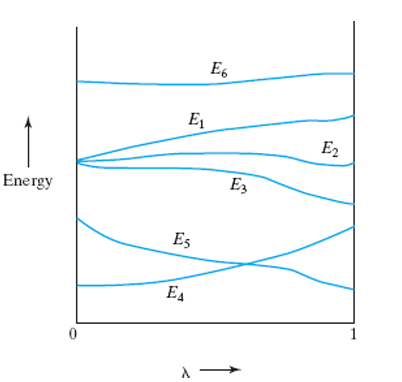
\includegraphics[width=0.4\textwidth]{Figures/9.2.png}
        \caption{微扰对能级的作用。}
        \label{fig:9.2}
    \end{figure}

    随着$\lambda \to 0$,满足(\ref{eq:9.69})的本征函数逐渐靠近满足(\ref{eq:9.67})的本征函数。这是否意味着$\lim_{\lambda \to 0} \psi_n $\\$= \psi_n^{\left(0\right)}$?不一定。若$E_n^{\left(0\right)}$是非简并的,则只有唯一的$\hat{H}^0$的归一化本征函数,其本征值为$E_n^{\left(0\right)}$,我们可以断定$\lim_{\lambda \to 0} \psi_n = \psi_n^{\left(0\right)}$。然而,当$E_n^{\left(0\right)}$是$d$重简并时,任何线性组合(第\ref{sec:3.6 Degeneracy}节)
    \begin{equation}
        c_1\psi_1^{\left(0\right)} + c_2\psi_2^{\left(0\right)} + \ldots + c_d\psi_d^{\left(0\right)}
        \label{eq:9.71}
    \end{equation}
    都是(\ref{eq:9.67})的解,本征值也为(\ref{eq:9.68})。线性无关的归一化函数集 $\psi_1^{\left(0\right)}, \psi_2^{\left(0\right)},\ldots,\psi_d^{\left(0\right)}$(我们将其用作对应于简并能级的本征函数)并不是唯一的。利用 (\ref{eq:9.71}) ,我们可以为简并能级构造出无穷多组由 $d$ 个线性无关的归一化特征函数构成的函数组。就未扰动问题而言,这样的集合与其他集合一样好。例如,对于氢原子三重简并的$2p$态,我们可以使用$2p_1$、$2p_0$和$2p_{-1}$作为基态函数,也可以使用$2p_x$、$2p_y$和$2p_z$,或其他一些由三个线性无关的函数组成的集合,这些函数是由前述集合的元素线性组合而成的。对于与 $d$ 重简并未扰动能级相对应的微扰本征函数,我们只能说,当 $\lambda$ 接近零时,它们各自接近非扰动特征函数的线性组合:
    \begin{equation}
        \lim_{\lambda \to 0} \psi_n = \sum_{i=1}^{d}c_1\psi_i^{\left(0\right)}, \quad 1 \leq n \leq d
        \label{eq:9.72}
    \end{equation}

    因此,我们第一个任务是确定微扰项$\hat{H}'$的\textbf{校正零级波函数(\ref{eq:9.72})}(correct zeroth-order wave functions)。回忆这些校正零级波函数$\phi_n^{\left(0\right)}$,我们有
    \begin{equation}
        \phi_n^{\left(0\right)} = \lim_{\lambda \to 0} \psi_n = \sum_{i=1}^{d}c_i\psi_i^{\left(0\right)}, \quad 1 \leq n \leq d
        \label{eq:9.73}
    \end{equation}
    每个不同的$\phi_n^{\left(0\right)}$在(\ref{eq:9.73})中都有一种不同的系数。校正零级波函数组取决于微扰项$\hat{H}'$的形式。

    对$d$重简并能级的处理过程与第\ref{sec:9.2 Nondegenerate Perturbation Theory}节的非简并微扰理论类似,不过,我们用$\phi_n^{\left(0\right)}$代替$\psi_n^{\left(0\right)}$。与(\ref{eq:9.13})和(\ref{eq:9.14})不同,我们有
    \begin{equation}
            \psi_n = \phi_n^{\left(0\right)} + \lambda\phi_n^{\left(1\right)} + \lambda^2\phi_n^{\left(2\right)} + \ldots, \quad n = 1,2,\ldots,d
            \label{eq:9.74}
    \end{equation}
    \begin{equation}
            E_n = E_n^{\left(0\right)} + \lambda E_n^{\left(1\right)} + \lambda^2 E_n^{\left(2\right)} + \ldots, \quad n = 1,2,\ldots,d
            \label{eq:9.75}
    \end{equation}
    其中用到了(\ref{eq:9.68})。将其带入$\hat{H}\psi_n = E_n\psi_n$,我们得到
    \begin{equation*}
        \begin{aligned}
            \left(\hat{H}^0 + \lambda\hat{H}'\right)&\left(\phi_n^{\left(0\right)} + \lambda\psi_n^{\left(1\right)} + \lambda^2\psi_n^{\left(2\right)} + \ldots\right) \\
            &= \left(E_d^{\left(0\right)} + \lambda E_n^{\left(1\right)} + \lambda^2 E_n^{\left(2\right)} + \ldots\right)\left(\phi_n^{\left(0\right)} + \lambda\psi_n^{\left(1\right)} + \lambda^2\psi_n^{\left(2\right)} + \ldots\right)
        \end{aligned}
    \end{equation*}
    令该方程中$\lambda^0$项的系数相等,我们得到$\hat{H}^0\phi_n^{\left(0\right)} = E_d^{\left(0\right)}\phi_n^{\left(0\right)}$。根据第\ref{sec:3.6 Degeneracy}节的理论,每个线性组合$\phi_n^{\left(0\right)}\left(n = 1,2,\ldots,d\right)$都是$\hat{H}^0$的本征函数,其本征值为$E_d^{\left(0\right)}$,该方程没有任何有用的信息。

    令$\lambda^1$项的系数相等,我们得到
    \begin{equation*}
        \hat{H}^0\psi_n^{\left(1\right)} + \hat{H}'\phi_n^{\left(0\right)} = E_d^{\left(0\right)}\psi_n^{\left(1\right)} + E_n^{\left(1\right)}\phi_n^{\left(0\right)}
    \end{equation*}
    \begin{equation}
        \hat{H}^{\left(0\right)}\psi_n^{\left(1\right)} - E_d^{\left(0\right)}\psi_n^{\left(1\right)} = E_n^{\left(1\right)}\phi_n^{\left(0\right)} - \hat{H}'\phi_n^{\left(0\right)}, \quad n = 1,2,\ldots,d
        \label{eq:9.76}
    \end{equation}
    将(\ref{eq:9.76})两边乘上$\phi_m^{\left(0\right)*}$并对全空间积分,其中,$m$ 是与所考虑的 $d$ 重简并未扰动能级相对应的状态之一;即$1 \leq m \leq d$。我们得到
    \begin{equation}
        \left\langle \psi_m^{\left(0\right)} \middle| \hat{H}^{\left(0\right)} \middle| \psi_n^{\left(1\right)} \right\rangle - E_d^{\left(0\right)} \left\langle \psi_m^{\left(0\right)} \middle| \psi_n^{\left(1\right)} \right\rangle = E^{\left(1\right)}\left\langle \psi_m^{\left(0\right)} \middle| \phi_n^{\left(0\right)} \right\rangle - \left\langle \psi_m^{\left(0\right)} \middle| \hat{H}' \middle| \phi_n^{\left(0\right)} \right\rangle, \quad n = 1,2,\ldots,d
        \label{eq:9.77}
    \end{equation}
    根据(\ref{eq:9.20}),我们有$\left\langle \psi_m^{\left(0\right)} \middle| \hat{H}^{\left(0\right)} \middle| \psi_n^{\left(1\right)} \right\rangle = E_n^{\left(0\right)}\left\langle \psi_m^{\left(0\right)} \middle| \psi_n^{\left(1\right)} \right\rangle$。根据(\ref{eq:9.68}),对于$1 \leq m \leq d$,我们有$E_d^{\left(0\right)} = E_n^{\left(0\right)}$,所以$\left\langle \psi_m^{\left(0\right)} \middle| \hat{H}^{\left(0\right)} \middle| \psi_n^{\left(1\right)} \right\rangle = E_d^{\left(0\right)}\left\langle \psi_m^{\left(0\right)} \middle| \psi_n^{\left(1\right)} \right\rangle$,(\ref{eq:9.77})的左侧为零。方程(\ref{eq:9.77})简化为
    \begin{equation*}
        \left\langle \psi_m^{\left(0\right)} \middle| \hat{H}' \middle| \phi_n^{\left(0\right)} \right\rangle - E_n^{\left(1\right)} \left\langle \psi_m^{\left(0\right)} \middle| \phi_n^{\left(0\right)} \right\rangle = 0, \quad m = 1,2,\ldots,d
    \end{equation*}
    将$\phi_n^{\left(0\right)}$的线性组合(\ref{eq:9.73})代入上式,我们得到
    \begin{equation}
        \sum_{i=1}^{d}c_i\left\langle \psi_m^{\left(0\right)} \middle| \hat{H}' \middle| \psi_i^{\left(0\right)} \right\rangle - E_n^{\left(1\right)} \sum_{i=1}^{d}c_i\left\langle \psi_m^{\left(0\right)} \middle| \psi_i^{\left(0\right)} \right\rangle = 0
        \label{eq:9.78}
    \end{equation}
    简并能级的零级波函数$\psi_i^{\left(0\right)}\left(i = 1,2,\ldots,d\right)$总是可以选择成为正交的,我们假设这点已经完成:
    \begin{equation}
        \left\langle \psi_m^{\left(0\right)} \middle| \psi_i^{\left(0\right)} \right\rangle = \delta_{mi}
        \label{eq:9.79}
    \end{equation}
    其中的$m$和$i$是从1到$d$的整数。(\ref{eq:9.78})变为
    \begin{equation}
        \sum_{i=1}^{d}\left[\left\langle \psi_m^{\left(0\right)} \middle| \hat{H}' \middle| \psi_i^{\left(0\right)} \right\rangle - E_n^{\left(1\right)}\delta_{mi}\right]c_i = 0, \quad m = 1,2,\ldots,d
        \label{eq:9.80}
    \end{equation}
    这是一组关于$d$个未知数$c_1, c_2, \ldots, c_d$的,由$d$个线性齐次方程组成的方程组,它们是(\ref{eq:9.73})中零级波函数的系数。我们可以将(\ref{eq:9.80})写全:
    \begin{equation}
        \begin{aligned}
            \left(H'_{11} - E_n^{\left(1\right)}\right)c_1 + H'_{12}c_2 + \ldots + H'_{1d}c_d &= 0 \\
            H'_{21}c_1 + \left(H'_{22} - E_n^{\left(1\right)}\right)c_2 + \ldots + H'_{2d}c_d &= 0 \\
            \ldots\ldots\ldots\ldots\ldots\ldots\ldots\ldots\ldots\ldots\ldots\ldots & \\
            H'_{d1}c_1 + H'_{d2}c_2 + \ldots + \left(H'_{dd} - E_n^{\left(1\right)}\right)c_d &= 0
        \end{aligned}
        \label{eq:9.81}
    \end{equation}
    \begin{eqnarray*}
        H'_{mi} \equiv \left\langle \psi_m^{\left(0\right)} \middle| \hat{H}' \middle| \psi_i^{\left(0\right)} \right\rangle
    \end{eqnarray*}
    若该线性齐次方程组有非平凡解,则系数行列式必须为零(第\ref{sec:8.4 Simultaneous Linear Equations}节):
    \begin{equation}
        \boxed{
            \det\left[\left\langle \psi_m^{\left(0\right)} \middle| \hat{H}' \middle| \psi_i^{\left(0\right)} \right\rangle - E_n^{\left(1\right)}\delta_{mi}\right] = 0
        }
        \label{eq:9.82}
    \end{equation}
    \begin{equation}
        \begin{vmatrix}
            H'_{11} - E_n^{\left(1\right)} & H'_{12} & \cdots & H'_{1d} \\
            H'_{21} & H'_{22} - E_n^{\left(1\right)} & \cdots & H'_{2d} \\
            \vdots & \vdots & \ddots & \vdots \\
            H'_{d1} & H'_{d2} & \cdots & H'_{dd} - E_n^{\left(1\right)}
        \end{vmatrix} = 0
        \label{eq:9.83}
    \end{equation}

    \textbf{久期方程}(\ref{eq:9.83})(secular equation)是关于$E_n^{\left(1\right)}$的$d$次代数方程。它有$d$个根,$E_1^{\left(1\right)}, E_2^{\left(1\right)}, \ldots, E_d^{\left(1\right)}$,是对 $d$ 重简并未扰动能级能量的一级校正。如果所有根都不同,那么微扰的一级校正就把 $d$ 重简并的未扰动能级分成了 $d$ 个不同的扰动能级(通过一级校正):
    \begin{equation*}
        E_d^{\left(0\right)} + E_1^{\left(1\right)}, \quad E_d^{\left(0\right)} + E_2^{\left(1\right)}, \quad \ldots, \quad E_d^{\left(0\right)} + E_d^{\left(1\right)}
    \end{equation*}
    如果久期方程的两个或更多根是相等的,则一级中简并能级未完全消除。在本节的剩余部分中,我们假设(\ref{eq:9.83})的所有根都是不同的。

    找到$d$个一级能量校正后,我们回到方程组(\ref{eq:9.81})来求未知数$c_i$,它决定了校正零级波函数。为了找到与根$E_n^{\left(1\right)}$相对应的校正零级波函数
    \begin{equation}
        \phi_n^{\left(0\right)} = c_1\psi_1^{\left(0\right)} + c_2\psi_2^{\left(0\right)} + \ldots + c_d\psi_d^{\left(0\right)}
        \label{eq:9.84}
    \end{equation}
    我们用$c_1$求解(\ref{eq:9.81})中的$c_2,c_3,\ldots,c_d$,随后通过归一化确定$c_1$。在(\ref{eq:9.79})中使用$\left\langle \phi^{\left(0\right)} \middle| \phi^{\left(0\right)} \right\rangle = 1$,我们得到(问题9.21)
    \begin{equation}
        \sum_{k=1}^{d}\left|c_k\right|^2 = 1
        \label{eq:9.85}
    \end{equation}
    对于每个根$E_n^{\left(1\right)}, \: n = 1,2,\ldots,d$,我们有一组不同的系数组$c_1, c_2, \ldots, c_d$,得到不同的校正零级波函数。

    在下一节中,我们将证明
    \begin{equation}
        E_n^{\left(1\right)} = \left\langle \phi_n^{\left(0\right)} \middle| \hat{H}' \middle| \phi_n^{\left(0\right)} \right\rangle, \quad n = 1,2,\ldots,d
        \label{eq:9.86}
    \end{equation}
    与非简并态的公式(\ref{eq:9.22})类似,不过需要使用校正零级波函数。

    利用与非简并情况类似的步骤,我们现在可以找到对校正零阶波函数的一级校正和二级能量校正。结果见\textit{Bates}, Volume I, pages 197–198; \textit{Hameka}, pages 230–231。

    举一个例子,考虑微扰项$\hat{H}'$作用于立方势箱中粒子最低的简并能级。我们有三个状态与该能级相对应:$\psi_{211}^{\left(0\right)}$、$\psi_{121}^{\left(0\right)}$和$\psi_{112}^{\left(0\right)}$。这些未扰动波函数是正交的,久期方程(\ref{eq:9.83})为
    \begin{equation}
        \begin{vmatrix}
            \left\langle 211 \middle| \hat{H}' \middle| 211 \right\rangle - E_n^{\left(1\right)} & \left\langle 211 \middle| \hat{H}' \middle| 121 \right\rangle & \left\langle 211 \middle| \hat{H}' \middle| 112 \right\rangle \\
            \left\langle 121 \middle| \hat{H}' \middle| 211 \right\rangle & \left\langle 121 \middle| \hat{H}' \middle| 121 \right\rangle - E_n^{\left(1\right)} & \left\langle 121 \middle| \hat{H}' \middle| 112 \right\rangle \\
            \left\langle 112 \middle| \hat{H}' \middle| 211 \right\rangle & \left\langle 112 \middle| \hat{H}' \middle| 121 \right\rangle & \left\langle 112 \middle| \hat{H}' \middle| 112 \right\rangle - E_n^{\left(1\right)}
        \end{vmatrix} = 0
        \label{eq:9.87}
    \end{equation}
    解出该方程,我们得到一级能量校正:$E_1^{\left(1\right)}$、$E_2^{\left(1\right)}$和$E_3^{\left(1\right)}$。三重简并的未扰动能级分裂为三个不同的能级(通过第一顺序):$\left(6h^2/8ma^2\right) + E_1^{\left(1\right)}$、$\left(6h^2/8ma^2\right) + E_2^{\left(1\right)}$、$\left(6h^2/8ma^2\right) + E_3^{\left(1\right)}$。分别使用根$E_1^{\left(1\right)}$、$E_2^{\left(1\right)}$和$E_3^{\left(1\right)}$,我们可以得到不同的方程组(\ref{eq:9.81})。求出每个方程,我们得到三组系数,它们决定了三个校正零级波函数。

    如果您对矩阵代数比较熟悉,可以注意到:求解(\ref{eq:9.83})和(\ref{eq:9.81})等价于求元素为$\left\langle \psi_m^{\left(0\right)} \middle| \hat{H}' \middle| \psi_i^{\left(0\right)} \right\rangle$的矩阵的本征值和本征向量。

\section{久期方程的简化}
\label{sec:9.6 Simplification of the Duration Equation}

    若久期行列式的某些非对角元素为零,则久期方程(\ref{eq:9.83})可以简化。在最有利的情况下,所有非对角元素都为零,久期方程变为
    \begin{equation}
        \begin{vmatrix}
            H'_{11} - E_n^{\left(1\right)} & 0 & \cdots & 0 \\
            0 & H'_{22} - E_n^{\left(1\right)} & \cdots & 0 \\
            \vdots & \vdots & \ddots & \vdots \\
            0 & 0 & \cdots & H'_{dd} - E_n^{\left(1\right)}
        \end{vmatrix} = 0
        \label{eq:9.88}
    \end{equation}
    \begin{equation*}
        \left(H'_{11} - E_n^{\left(1\right)}\right)\left(H'_{22} - E_n^{\left(1\right)}\right)\cdots\left(H'_{dd} - E_n^{\left(1\right)}\right) = 0
    \end{equation*}
    \begin{equation}
        E_1^{\left(1\right)} = H'_{11}, \quad E_2^{\left(1\right)} = H'_{22}, \quad \ldots, \quad E_d^{\left(1\right)} = H'_{dd}
        \label{eq:9.89}
    \end{equation}
    现在我们想知道零级校正波函数。假设(\ref{eq:9.89})的根都是不同的。对于根$E_n^{\left(1\right)} = H'_{11}$方程组(\ref{eq:9.81})为
    \begin{equation*}
        \begin{aligned}
            0 &= 0 \\
            \left(H'_{22} - H'_{11}\right) c_2 &= 0 \\
            \ldots\ldots\ldots\ldots & \ldots \\
            \left(H'_{dd} - H'_{11}\right) c_d &= 0
        \end{aligned}
    \end{equation*}
    由于我们假设所有根都不相等,则$H'_{22} - H'_{11}, H'_{33} - H'_{11}, \ldots, H'_{dd} - H'_{11}$都不为零,因此$c_2 = c_3 = \ldots = c_d = 0$。归一化条件(\ref{eq:9.85})给出$c_1 = 1$。对应于能量一级微扰校正$H'_{11}$的零级校正波函数为[式(\ref{eq:9.73})]$\phi_1^{\left(0\right)} = \psi_1^{\left(0\right)}$。对于根$H'_{22}$,同样的理由给出$\phi_2^{\left(0\right)} = \psi_2^{\left(0\right)}$。\textit{若久期行列式为对角行列式,则最初假设的波函数$\psi_1^{\left(0\right)}, \psi_2^{\left(0\right)}, \ldots, \psi_d^{\left(0\right)}$就是微扰$\hat{H}'$的零级校正波函数。}

    反之亦然。若最初假设的波函数是零级校正波函数,则久期行列式的非对角元素为零。具体情况如下。由$\phi_1^{\left(0\right)} = \psi_1^{\left(0\right)}$我们得知,展开式$\phi_1^{\left(0\right)} = \sum_{i=1}^{d}c_i\psi_i^{\left(0\right)}$中,$c_1 = 1$,$c_2 = c_3 = \ldots = c_d = 0$,所以若$n=1$,则方程组(\ref{eq:9.81})变为
    \begin{equation*}
        H'_{11}c_1 - E_1^{\left(1\right)} = 0, \quad H'_{21} = 0, \quad \ldots, \quad H'_{d1} = 0
    \end{equation*}
    将同样地推理应用于剩余的函数$\phi_n^{\left(0\right)}$,得出对$i \neq m$,有$H'_{mi} = 0$。因此,零级校正波函数的使用使得久期行列式得以对角化。还需要注意的是,通过对零级校正波函数的微扰求平均值,可以得到能量的一级校正:
    \begin{equation}
        E_n^{\left(1\right)} = H'_{nn} = \left\langle \phi_n^{\left(0\right)} \middle| \hat{H}' \middle| \phi_n^{\left(0\right)} \right\rangle
        \label{eq:9.90}
    \end{equation}

    通常,久期行列式不是对角形式,而是块对角形式。例如,我们可能有
    \begin{equation}
        \begin{vmatrix}
            H'_{11} - E_n^{\left(1\right)} & H'_{12} & 0 & 0 \\
            H'_{21} & H'_{22} - E_n^{\left(1\right)} & 0 & 0 \\
            0 & 0 & H'_{33} - E_n^{\left(1\right)} & H'_{34} \\
            0 & 0 & H'_{43} & H'_{44} - E_n^{\left(1\right)}
        \end{vmatrix} = 0
        \label{eq:9.91}
    \end{equation}
    (\ref{eq:9.91})中的久期行列式与带有$S_{ij} = \delta_{ij}$的线性变分久期方程(\ref{eq:8.65})中久期行列式的形式相同。根据同样的推理过程,可以得出:两个变分函数是$f_1$和$f_2$的线性组合,两个是$f_3$和$f_4$的线性组合,因此两个零级校正波函数是$\psi_1^{\left(0\right)}$和$\psi_2^{\left(0\right)}$的线性组合,另两个是$\psi_3^{\left(0\right)}$和$\psi_4^{\left(0\right)}$的线性组合:
    \begin{equation*}
        \phi_1^{\left(0\right)} = c_1\psi_1^{\left(0\right)} + c_2\psi_2^{\left(0\right)}, \quad \phi_2^{\left(0\right)} = c_1'\psi_1^{\left(0\right)} + c_2'\psi_2^{\left(0\right)}
    \end{equation*}
    \begin{equation*}
        \phi_3^{\left(0\right)} = c_3\psi_3^{\left(0\right)} + c_4\psi_4^{\left(0\right)}, \quad \phi_4^{\left(0\right)} = c_3'\psi_3^{\left(0\right)} + c_4'\psi_4^{\left(0\right)}
    \end{equation*}
    其中$'$符号用于表示不同的系数。

    \textit{ 当简并微扰理论的久期行列式为块对角形式时,久期方程会分解为两个或多个较小的久期方程,系数$c_i$的联立方程组(\ref{eq:9.81})也会分解为两个或多个较小的联立方程组。}

    相反地,如果我们有一个四重简并的未扰动能级,且恰好知道$\phi_1^{\left(0\right)}$和$\phi_2^{\left(0\right)}$都只是$\psi_1^{\left(0\right)}$和$\psi_2^{\left(0\right)}$的线性组合,而$\phi_3^{\left(0\right)}$和$\phi_4^{\left(0\right)}$只是$\psi_3^{\left(0\right)}$和$\psi_4^{\left(0\right)}$的线性组合,则我们处理的是两个二阶久期行列式,而不是一个四阶久期行列式。

    如何事先选择正确的零级波函数,从而简化久期方程?假设有一算符$\hat{A}$同时与$\hat{H}^0$和$\hat{H}'$对易。我们可以选择未扰动波函数为$\hat{A}$的本征函数。由于$\hat{A}$与$\hat{H}^0$对易,若$\psi_i^{\left(0\right)}$和$\psi_j^{\left(0\right)}$对应于算符$\hat{A}$的不同本征值[见式(\ref{eq:7.50})],则未扰动函数的选择将使积分$H'_{ij}$消失。因此,若$\hat{A}$的本征函数$\psi_1^{\left(0\right)}, \psi_2^{\left(0\right)}, \ldots, \psi_d^{\left(0\right)}$对应于不同的本征值,则久期行列式为对角形式,我们就得到了正确的零级波函数。若$\hat{A}$的某些本征值是相同的,我们就得到了块对角而不是纯对角形式的久期行列式。一般来说,正确的零级函数将是具有相同 $\hat{A}$ 本征值的未扰动函数的线性组合。(这是意料之中的,因为$\hat{H}$与$\hat{H} = \hat{H}^0 + \lambda\hat{H}'$对易,所以$\hat{H}$的微扰本征函数可以选择成为$\hat{A}$的本征函数。)例子见问题9.23。

\section{微扰理论处理氦原子第一激发态}
\label{sec:9.7 Perturbation Treatment of the First Excited State of Helium}

    第\ref{sec:9.3 Perturbation Treatment of the Helium-Atom Ground State}节中,我们已经使用微扰理论处理了氦原子基态。现在我们将处理氦原子第一激发态。未扰动能量由(\ref{eq:9.48})给出。最低未扰动激发态满足$n_1 = 1, n_2 = 2$或$n_1 = 2, n_2 = 1$,带入(\ref{eq:9.48}),我们得到
    \begin{equation}
        E_n^{\left(0\right)} = -\frac{5Z^2}{8}\left(\frac{\mathrm{e}^2}{4\pi\varepsilon_0a_0}\right) = -\frac{20}{8}2\left(\frac{\mathrm{e}^2}{8\pi\varepsilon_0a_0}\right) = -5\left(13.606 \:\mathrm{eV}\right) = -68.03 \:\mathrm{eV}
        \label{eq:9.92}
    \end{equation}
    回忆:类氢原子的$n=2$能级是四重简并的,$2s$和三个$2p$态都具有相同的能量值。\ce{He}原子第一未扰动激发态的能级是八重简并的。八个未扰动波函数为[式(\ref{eq:9.44})]:
    \begin{equation}
        \begin{aligned}
            \psi_1^{\left(0\right)} &= 1s\left(1\right)2s\left(2\right), \quad \psi_2^{\left(0\right)} = 2s\left(1\right)1s\left(2\right), \quad \psi_3^{\left(0\right)} = 1s\left(1\right)2p_x\left(2\right), \quad \psi_4^{\left(0\right)} = 2p_x\left(1\right)1s\left(2\right) \\
            \psi_5^{\left(0\right)} &= 1s\left(1\right)2p_y\left(2\right), \quad \psi_6^{\left(0\right)} = 2p_y\left(1\right)1s\left(2\right), \quad \psi_7^{\left(0\right)} = 1s\left(1\right)2p_z\left(2\right), \quad \psi_8^{\left(0\right)} = 2p_z\left(1\right)1s\left(2\right)
        \end{aligned}
        \label{eq:9.93}
    \end{equation}
    其中$1s\left(1\right)2s\left(2\right)$表示电子1的类氢函数$1s$和电子2的类氢函数$2s$的乘积。例如$\psi_8^{\left(0\right)}$的显式形式如下(表\ref{tab:6.2}):
    \begin{equation*}
        \psi_8^{\left(0\right)} = \frac{1}{4\left(2\pi\right)^{1/2}}\left(\frac{Z}{a_0}\right)^{5/2}r_1\mathrm{e}^{-Zr_1/2a_0}\cos\theta_1 \cdot \frac{1}{\pi^{1/2}}\left(\frac{Z}{a_0}\right)^{3/2}r_2^2\mathrm{e}^{-Zr_2/a_0}
    \end{equation*}
    我们选择使用实$2p$类氢轨道,而不是其他复函数轨道。

    由于未扰动能级是简并的,我们必须求解久期方程。久期方程(\ref{eq:9.83})假设函数$\psi_1^{\left(0\right)}, \psi_2^{\left(0\right)}, \ldots, \psi_8^{\left(0\right)}$是正交的。该条件已经满足。例如,
    \begin{equation*}
        \begin{aligned}
            \int \psi_1^{\left(0\right)*}\psi_1^{\left(0\right)}\mathrm{d}\tau &= \int\int 1s\left(1\right)^*2s\left(2\right)^*1s\left(1\right)2s\left(2\right)\:\mathrm{d}\tau_1\:\mathrm{d}\tau_2 \\
            &= \int \left|1s\left(1\right)\right|^2 \:\mathrm{d}\tau_1 \int \left|2s\left(2\right)\right|^2 \:\mathrm{d}\tau_2 = 1 \cdot 1 = 1 \\ 
            \int \psi_3^{\left(0\right)*}\psi_5^{\left(0\right)}\:\mathrm{d}\tau &= \int \left|1s\left(1\right)\right|^2 \:\mathrm{d}\tau_1 \int 2p_x\left(2\right)^*2p_y\left(2\right)\:\mathrm{d}\tau_2 = 1 \cdot 0 = 0
        \end{aligned}
    \end{equation*}
    其中用到了类氢轨道的正交性。

    久期行列式包含$8^2 = 64$个元素。算符$\hat{H}'$是厄米算符,$H_{ij}' = \left(H_{ji}'\right)^*$。同样地,由于$\hat{H}'$是实算符,$\psi_1^{\left(0\right)},\ldots, \psi_8^{\left(0\right)}$是实函数,我们有$\left(H_{ji}'\right)^* = H_{ij}'$,即$H_{ij}' = H_{ji}'$。久期行列式关于主对角线对称。 这样一来,求积分的工作量几乎就减少了一半。

    考虑使用宇称,可以证明:大部分的积分$H_{ij}'$为零。首先,考虑$H_{13}'$:
    \begin{equation*}
        H_{13}' = \int_{-\infty}^{\infty} \int_{-\infty}^{\infty} \int_{-\infty}^{\infty} \int_{-\infty}^{\infty} \int_{-\infty}^{\infty} \int_{-\infty}^{\infty} 1s\left(1\right)2s\left(2\right)\frac{\mathrm{e}^2}{4\pi\varepsilon_0r_{12}}1s\left(1\right)2p_x\left(2\right)\:\mathrm{d}x_1\:\mathrm{d}y_1\:\mathrm{d}z_1\:\mathrm{d}x_2\:\mathrm{d}y_2\:\mathrm{d}z_2
    \end{equation*}
    类氢函数$s$只依赖于$r = \left(x^2+y^2+z^2\right)^{1/2}$,因此是偶函数。$2p_x\left(2\right)$是$x_2$的奇函数[式(\ref{eq:6.119})]。$r_{12}$由(\ref{eq:9.66})给出,如果我们将六个坐标反转,$r_{12}$保持不变:
    \begin{equation*}
        r_{12} \to \left[\left(-x_1+x_2\right)^2 + \left(-y_1+y_2\right)^2 + \left(-z_1+z_2\right)^2\right]^{1/2} = r_{12}
    \end{equation*}
    因此,反转六个坐标,积分$H_{13}'$变为其相反数。那么[式(\ref{eq:7.74})],$H_{13}' = 0$。同样地,$H_{14}' = H_{15}' = H_{16}' = H_{17}' = H_{18}' = 0$;$H_{23}' = H_{24}' = H_{25}' = H_{26}' = H_{27}' = H_{28}' = 0$。现在考虑$H_{35}'$:
    \begin{equation*}
        H_{35}' = \int_{-\infty}^{\infty} \cdots \int_{-\infty}^{\infty} 1s\left(1\right)2p_x\left(2\right)\frac{\mathrm{e}^2}{4\pi\varepsilon_0r_{12}}1s\left(1\right)2p_y\left(2\right)\:\mathrm{d}x_1\cdots\mathrm{d}z_2
    \end{equation*}
    假设我们反转$x$坐标:$x_1 \to -x_1$,$x_2 \to -x_2$。该操作未改变$r_{12}$,$1s\left(1\right)$和$2p_y\left(2\right)$也不受影响。然而,$2p_x\left(2\right)$变为其相反数,因此,净效果是将$H_{35}'$变为其相反数。所以(问题7.30),$H_{35}' = 0$。同样地,$H_{36}' = H_{37}' = H_{38}' = 0$;$H_{45}' = H_{46}' = H_{47}' = H_{48}' = 0$。同样反转$y_1 \to -y_1$和$y_2 \to -y_2$,我们得到$H_{57}' = H_{58}' = H_{67}' = H_{68}' = 0$。久期方程变为
    \begin{equation*}
        \begin{vmatrix}
            b_{11} & H_{12}' & 0 & 0 & 0 & 0 & 0 & 0 \\
            H_{12}' & b_{22} & 0 & 0 & 0 & 0 & 0 & 0 \\
            0 & 0 & b_{33} & H_{34}' & 0 & 0 & 0 & 0 \\
            0 & 0 & H_{34}' & b_{44} & 0 & 0 & 0 & 0 \\
            0 & 0 & 0 & 0 & b_{55} & H_{56}' & 0 & 0 \\
            0 & 0 & 0 & 0 & H_{56}' & b_{66} & 0 & 0 \\
            0 & 0 & 0 & 0 & 0 & 0 & b_{77} & H_{78}' \\
            0 & 0 & 0 & 0 & 0 & 0 & H_{78}' & b_{88}
        \end{vmatrix} = 0
    \end{equation*}
    \begin{equation*}
        b_{ii} \equiv H_{ii}' - E^{\left(1\right)}, \quad i = 1,2,\ldots,8
    \end{equation*}

    久期行列式为块对角行列式,可以分解为四个行列式,每个二阶。可以得出零级校正波函数具有如下形式:
    \begin{equation}
        \begin{aligned}
            \phi_1^{\left(0\right)} &= c_1\psi_1^{\left(0\right)} + c_2\psi_2^{\left(0\right)}, \quad \phi_2^{\left(0\right)} = \bar{c}_1\psi_1^{\left(0\right)} + \bar{c}_2\psi_2^{\left(0\right)} \\
            \phi_3^{\left(0\right)} &= c_3\psi_3^{\left(0\right)} + c_4\psi_4^{\left(0\right)}, \quad \phi_4^{\left(0\right)} = \bar{c}_3\psi_3^{\left(0\right)} + \bar{c}_4\psi_4^{\left(0\right)} \\
            \phi_5^{\left(0\right)} &= c_5\psi_5^{\left(0\right)} + c_6\psi_6^{\left(0\right)}, \quad \phi_6^{\left(0\right)} = \bar{c}_5\psi_5^{\left(0\right)} + \bar{c}_6\psi_6^{\left(0\right)} \\
            \phi_7^{\left(0\right)} &= c_7\psi_7^{\left(0\right)} + c_8\psi_8^{\left(0\right)}, \quad \phi_8^{\left(0\right)} = \bar{c}_7\psi_7^{\left(0\right)} + \bar{c}_8\psi_8^{\left(0\right)}
        \end{aligned}
        \label{eq:9.94}
    \end{equation}
    其中,未加横杠的系数对应于每个二阶行列式的一个根,加横杠的系数对应于第二个根。

    第一个行列式为
    \begin{equation}
        \begin{vmatrix}
            H_{11}' - E^{\left(1\right)} & H_{12}' \\
            H_{21}' & H_{22}' - E^{\left(1\right)}
        \end{vmatrix} = 0
        \label{eq:9.95}
    \end{equation}
    我们有
    \begin{equation*}
        \begin{aligned}
            H_{11}^{\prime} & =\int_{-\infty}^{\infty} \ldots \int_{-\infty}^{\infty} 1 s(1) 2 s(2) \frac{e^{2}}{4 \pi \varepsilon_{0} r_{12}} 1 s(1) 2 s(2) \:\mathrm{d} x_{1} \ldots\: \mathrm{d} z_{2} \\
            H_{11}^{\prime} & =\int\int[1 s(1)]^{2}[2 s(2)]^{2} \frac{e^{2}}{4 \pi \varepsilon_{0} r_{12}} \:\mathrm{d} \tau_{1}\: \mathrm{d} \tau_{2} \\
            H_{22}^{\prime} & =\int\int[1 s(2)]^{2}[2 s(1)]^{2} \frac{e^{2}}{4 \pi \varepsilon_{0} r_{12}} \:\mathrm{d} \tau_{1} \:\mathrm{d} \tau_{2}
        \end{aligned}
    \end{equation*}
    积分变量是虚拟变量,可以用任何符号表示。我们使用如下方法标记$H_{22}'$中的积分:交换$x_1$和$x_2$,$y_1$和$y_2$,$z_1$和$z_2$。该过程没有改变$r_{12}$[式(\ref{eq:9.66})],因此
    \begin{equation}
        H'_{22} = \int [1s\ (1)]^2 [2s\ (2)]^2 \frac{\mathrm{e}^2}{4\pi\epsilon_0 r_{12}}\: \mathrm{d}\tau_2\: \mathrm{d}\tau_1 = H'_{11}
        \label{eq:9.96}
    \end{equation}
    同样的论证表明$H_{33}' = H_{44}'$,$H_{55}' = H_{66}'$,$H_{77}' = H_{88}'$。

    我们使用符号$J_{1s2s}$表示积分$H_{11}'$:
    \begin{equation}
        H_{11}' = J_{1s2s} = \int [1s\,(1)]^2 [2s\,(2)]^2 \frac{\mathrm{e}^2}{4\pi \epsilon_0 r_{12}}\: \mathrm{d}\tau_1\: \mathrm{d}\tau_2
        \label{eq:9.97}
    \end{equation}
    这是一个\textbf{库伦积分}(Coulomb integral)的例子,之所以叫库伦积分,是因为 $J_{1s2s}$ 等于概率密度函数为 $\left[1s\right]^2$ 的电子和概率密度函数为 $\left[2s\right]^2$ 的电子之间的静电排斥能。

    积分$H_{12}'$用$K_{1s2s}$表示:
    \begin{equation}
        H'_{12} = K_{1s2s} = \int 1s\left(1\right)2s\left(2\right) \frac{\mathrm{e}^2}{4\pi\varepsilon_0r_{12}} 2s\left(1\right)1s\left(2\right)\: \mathrm{d}\tau_1 \:\mathrm{d}\tau_2
        \label{eq:9.98}
    \end{equation}
    这是一个\textbf{交换积分}(exchange integral):$\frac{\mathrm{e}^2}{4\pi\varepsilon_0r_{12}}$左右两侧的积分之间的区别在于电子 1 和电子 2 的交换。

    库伦积分$J_{mn}$和交换积分$K_{mn}$的一般定义如下:
    \begin{equation}
        J_{mn} \equiv \left\langle f_m(1) f_n(2) \middle| \mathrm{e}^2/4\pi\varepsilon_0 r_{12} \middle| f_m(1) f_n(2) \right\rangle
        \label{eq:9.99}
    \end{equation}
    \begin{equation}
        K_{mn} \equiv \left\langle f_m(1) f_n(2) \middle| \mathrm{e}^2/4\pi\varepsilon_0 r_{12} \middle| f_n(1) f_m(2) \right\rangle
        \label{eq:9.100}
    \end{equation}
    其中的积分是对电子1和2的全空间坐标进行积分,$f_m$和$f_n$是空间轨道。

    将(\ref{eq:9.96})到(\ref{eq:9.98})带入(\ref{eq:9.95}),我们得到
    \begin{equation}
        \begin{vmatrix}
            J_{1s2s} - E^{\left(1\right)} & K_{1s2s} \\
            K_{1s2s} & J_{1s2s} - E^{\left(1\right)}
        \end{vmatrix} = 0
        \label{eq:9.101}
    \end{equation}
    \begin{equation*}
        \left(J_{1s2s} - E^{\left(1\right)}\right)^2 = K_{1s2s}^2
    \end{equation*}
    \begin{equation}
        E_1^{\left(1\right)} = J_{1s2s} - K_{1s2s}, \quad E_2^{\left(1\right)} = J_{1s2s} + K_{1s2s}
        \label{eq:9.102}
    \end{equation}

    现在我们寻找对应于这两个根的零级校正波函数的系数。在(\ref{eq:9.81})中使用$E_{1}^{\left(1\right)}$,得到
    \begin{equation*}
        \begin{aligned}
            K_{1s2s}c_1 + K_{1s2s}c_2 &= 0 \\
            K_{1s2s}c_1 + K_{1s2s}c_2 &= 0
        \end{aligned}
    \end{equation*}
    因此$c_2 = -c_1$。根据归一化条件,有
    \begin{equation*}
        \left\langle \phi_1^{(0)} \middle| \phi_1^{(0)} \right\rangle = \left\langle c_1 \psi_1^{(0)} - c_1 \psi_2^{(0)} \middle| c_1 \psi_1^{(0)} - c_1 \psi_2^{(0)} \right\rangle = |c_1|^2 + |c_1|^2 = 1
    \end{equation*}
    \begin{equation*}
        c_1 = 2^{-1/2}
    \end{equation*}
    其中我们用到了$\psi_1^{(0)}$和$\psi_2^{(0)}$的正交性。对应于$E_1^{(1)}$的零级校正波函数为
    \begin{equation}
        \phi_{1}^{(0)} = 2^{-1/2} \left(\psi_{1}^{(0)} - \psi_{2}^{(0)}\right) = 2^{-1/2} \left[ 1s(1)2s(2) - 2s(1)1s(2) \right]
        \label{eq:9.103}
    \end{equation}

    同样地,我们可以得到对应于$E_2^{(1)}$的零级校正波函数:
    \begin{equation}
        \phi_{2}^{(0)} = 2^{-1/2} \left(\psi_{1}^{(0)} + \psi_{2}^{(0)}\right) = 2^{-1/2} \left[ 1s(1)2s(2) + 2s(1)1s(2) \right]
        \label{eq:9.104}
    \end{equation}

    我们还有三个二阶行列式需要处理:
    \begin{equation}
        \begin{vmatrix}
            H_{33}' - E^{\left(1\right)} & H_{34}' \\
            H_{34}' & H_{44}' - E^{\left(1\right)}
        \end{vmatrix} = 0
        \label{eq:9.105}
    \end{equation}
    \begin{equation}
        \begin{vmatrix}
            H_{55}' - E^{\left(1\right)} & H_{56}' \\
            H_{56}' & H_{66}' - E^{\left(1\right)}
        \end{vmatrix} = 0
        \label{eq:9.106}
    \end{equation}
    \begin{equation}
        \begin{vmatrix}
            H_{77}' - E^{\left(1\right)} & H_{78}' \\
            H_{78}' & H_{88}' - E^{\left(1\right)}
        \end{vmatrix} = 0
        \label{eq:9.107}
    \end{equation}
    考虑$H_{33}'$和$H_{55}'$:
    \begin{equation*}
        \begin{aligned}
            H_{33}' &= \int_{-\infty}^{\infty}\cdots\int_{-\infty}^{\infty} 1s(1)2p_x(2)\frac{\mathrm{e}^2}{4\pi\varepsilon_0r_{12}} 1s(1)2p_x(2)\:\mathrm{d}x_1\cdots\mathrm{d}z_2 \\
            H_{55}' &= \int_{-\infty}^{\infty}\cdots\int_{-\infty}^{\infty} 1s(1)2p_y(2)\frac{\mathrm{e}^2}{4\pi\varepsilon_0r_{12}} 1s(1)2p_y(2)\:\mathrm{d}x_1\cdots\mathrm{d}z_2
        \end{aligned}
    \end{equation*}
    这两个积分是相等的——它们唯一的区别是将$2p_x\left(2\right)$替换为$2p_y\left(2\right)$——这两个轨道只是空间取向不同。更正式地说,如果我们根据方案$x_2 \to y_2, y_2 \to x_2, x_1 \to y_1, y_1 \to x_1$对 $H_{33}'$ 中的虚拟积分变量进行重新标注,那么$r_{12}$保持不变,则$H_{33}'$变为$H_{55}'$。同样地理由表明$H_{77}' = H_{33}'$。在这些库伦积分中引入符号$J_{1s2p}$,我们有:
    \begin{equation*}
        H'_{33} = H'_{55} = H'_{77} = J_{1s2p} = \int\int 1s(1)2p_z(2)\frac{\mathrm{e}^2}{4\pi\varepsilon_0 r_{12}}1s(1)2p_z(2) \:\mathrm{d}\tau_1\: \mathrm{d}\tau_2
    \end{equation*}
    同样地,有关$2p$轨道的交换积分也相等:
    \begin{equation*}
        H'_{34} = H'_{56} = H'_{78} = K_{1s2p} = \int\int 1s(1)2p_z(2)\frac{\mathrm{e}^2}{4\pi\varepsilon_0 r_{12}}2p_z(1)1s(2)\:\mathrm{d}\tau_1\: \mathrm{d}\tau_2
    \end{equation*}
    因此,(\ref{eq:9.105}) 至 (\ref{eq:9.107}) 三个行列式完全相同,其形式为
    \begin{equation*}
        \begin{vmatrix}
            J_{1s2p} - E^{\left(1\right)} & K_{1s2p} \\
            K_{1s2p} & J_{1s2p} - E^{\left(1\right)}
        \end{vmatrix} = 0
    \end{equation*}
    该行列式与(\ref{eq:9.101})相似,类比 (\ref{eq:9.102})-(\ref{eq:9.104}) 可得
    \begin{equation}
        E_{3}^{\left(1\right)} = E_{5}^{\left(1\right)} = E_7^{\left(1\right)} = J_{1s2p} - K_{1s2p}
        \label{eq:9.108}
    \end{equation}
    \begin{equation}
        E_{4}^{\left(1\right)} = E_{6}^{\left(1\right)} = E_8^{\left(1\right)} = J_{1s2p} + K_{1s2p}
        \label{eq:9.109}
    \end{equation}
    \begin{equation}
        \begin{aligned}
            \phi_3^{\left(0\right)} &= 2^{-1/2}\left[1s\left(1\right)2p_x\left(2\right) - 1s\left(2\right)2p_x\left(1\right)\right] \\
            \phi_4^{\left(0\right)} &= 2^{-1/2}\left[1s\left(1\right)2p_x\left(2\right) + 1s\left(2\right)2p_x\left(1\right)\right] \\
            \phi_5^{\left(0\right)} &= 2^{-1/2}\left[1s\left(1\right)2p_y\left(2\right) - 1s\left(2\right)2p_y\left(1\right)\right] \\
            \phi_6^{\left(0\right)} &= 2^{-1/2}\left[1s\left(1\right)2p_y\left(2\right) + 1s\left(2\right)2p_y\left(1\right)\right] \\
            \phi_7^{\left(0\right)} &= 2^{-1/2}\left[1s\left(1\right)2p_z\left(2\right) - 1s\left(2\right)2p_z\left(1\right)\right] \\
            \phi_8^{\left(0\right)} &= 2^{-1/2}\left[1s\left(1\right)2p_z\left(2\right) + 1s\left(2\right)2p_z\left(1\right)\right]
        \end{aligned}
        \label{eq:9.110}
    \end{equation}

    电子间排斥势$\mathrm{e}^2/4\pi\varepsilon_0 r_{12}$部分消除了简并的现象。假设的八重简并未扰动能级裂分为与组态$1s2s$相关的两个非简并能级和两个与组态$2s2p$相关的三重简并能级。人们可能认为,高级能量校正会进一步解决简并问题。事实上,要完全消除简并,需要施加外磁场。由于微扰$\mathrm{e}/4\pi\varepsilon_0a_0$项未完全消除简并,任何$\phi_3^{\left(0\right)},\phi_5^{\left(0\right)},\phi_7^{\left(0\right)}$的归一化线性组合和$\phi_4^{\left(0\right)},\phi_6^{\left(0\right)},\phi_8^{\left(0\right)}$的归一化线性组合都可以是零级校正波函数。

    为了计算(\ref{eq:9.102})和(\ref{eq:9.108})中的库伦积分和交换积分,我们使用问题9.14中给出的$1/r_{12}$的展开式。结果为
    \begin{equation}
        \begin{aligned}
            J_{1s2s} &= \left( \frac{17}{81} \right) \frac{Ze^2}{4\pi \varepsilon_0 a_0} = 11.42 \:\mathrm{eV}, \quad J_{1s2p} = \left( \frac{59}{243} \right) \frac{Ze^2}{4\pi \varepsilon_0 a_0} = 13.21 \:\mathrm{eV} \\
            K_{1s2s} &= \left(\frac{16}{729}\right) \frac{Ze^2}{4\pi \varepsilon_0 a_0} = 1.19 \:\mathrm{eV}, \quad K_{1s2p} = \left(\frac{112}{6561}\right) \frac{Ze^2}{4\pi \varepsilon_0 a_0} = 0.93\:\mathrm{eV}
        \end{aligned}
        \label{eq:9.111}
    \end{equation}
    其中$Z=2$,$\mathrm{e}^2/4\pi\varepsilon_0 a_0 = 13.606 \:\mathrm{eV}$。回忆$E^{\left(0\right)} = -68.03 \:\mathrm{eV}$,我们得到(图\ref{fig:9.3}):
    \begin{figure}[ht]
        \centering
        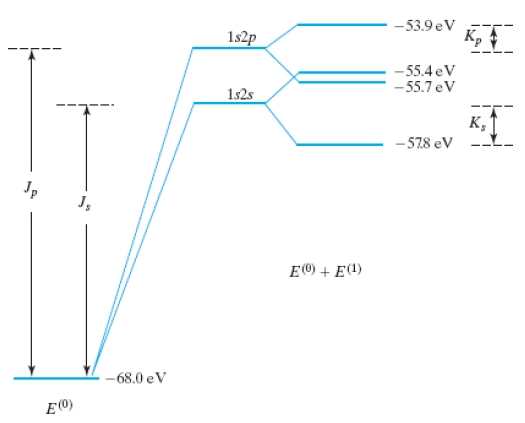
\includegraphics[width=0.5\textwidth]{Figures/9.3.png}
        \caption{氦原子第一激发态。}
        \label{fig:9.3}
    \end{figure}
    \begin{equation*}
        \begin{aligned}
            E^{(0)} + E_1^{(1)} &= E^{(0)} + J_{1s2s} - K_{1s2s} = -57.8 \:\mathrm{eV} \\
            E^{(0)} + E_2^{(1)} &= E^{(0)} + J_{1s2s} + K_{1s2s} = -55.4 \:\mathrm{eV} \\
            E^{(0)} + E_3^{(1)} &= E^{(0)} + J_{1s2p} - K_{1s2p} = -55.75 \:\mathrm{eV} \\
            E^{(0)} + E_4^{(1)} &= E^{(0)} + J_{1s2p} + K_{1s2p} = -53.9 \:\mathrm{eV}
        \end{aligned}
    \end{equation*}
    能量的一级校正似乎表明:组态$1s2p$的两个较低的能级能量比$1s2s$组态两个较高能级的能量低。对氦光谱的研究表明,事实并非如此。该误差由忽略能量的高级微扰校正造成。

    Knight和Scherr使用变分-微扰法(第 \ref{sec:9.2 Nondegenerate Perturbation Theory} 节)计算了这四个激发水平的二级和三级校正 $E^{(2)}$ 和 $E^{(3)}$。[R. E. Knight and C. W. Scherr, \textit{Rev. Mod. Phys.}, \textbf{35}, 431 (1963).十七级能量校正见F. C. Sanders and C. W. Scherr, \textit{Phys. Rev.}, \textbf{181}, 84 (1969).]图\ref{fig:9.4}展示了他们的成果(与实验值相差$0.1 \: \mathrm{eV}$)。图\ref{fig:9.4}表明图\ref{fig:9.3}并不准确。因为微扰项$\mathrm{e}^2/4\pi\varepsilon_0 r_{12}$并不真的很小,只包含$E^{\left(1\right)}$校正的微扰处理无法给出准确的结果。
    \begin{figure}
        \centering
        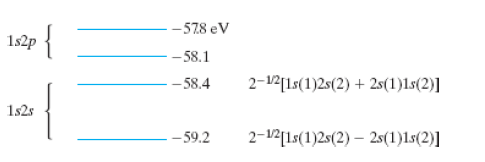
\includegraphics[width=0.65\textwidth]{Figures/9.4.png}
        \caption{
            \centering
            \parbox{0.4\linewidth}{
                \noindent
                \ce{He}第一激发态的$E^{\left(0\right)} + E_{\left(1\right)} + E_{\left(2\right)} + E_{\left(3\right)}$能量。 同时展示了$1s2s$能级的零级校正波函数。
            }
        }
        \label{fig:9.4}
    \end{figure}

    波函数的一级校正$\psi^{\left(1\right)}$引入了其他组态的贡献(组态相互作用)。当我们说某个能级属于组态$1s2s$时,我们指出的是对真实波函数贡献最大的组态。

    我们从八个简并的零级波函数(\ref{eq:9.93})开始。这些函数有三种兼并方式。一是具有相同$n$但不同$l$值的类氢函数之间的简并,$2s$和$2p$函数具有相同的能量。二是相同$n$和$l$但不同$m$值之间的简并,$2p_1,2p_0,2p_{-1}$函数具有相同的能量。(方便起见,我们使用实际波函数$2p_{x,y,z}$,但是我们可以从函数$2p_{1,0,-1}$开始。)最后,是仅在轨道间两个电子的交换上不同的函数之间的简并(全同粒子,译者注);函数$\psi_1^{\left(0\right)} = 1s\left(1\right)2s\left(2\right)$和$\psi_2^{\left(0\right)} = 1s\left(2\right)2s\left(1\right)$有相同的能量。最后一种简并形式称为\textit{交换简并}(exchange degeneracy)。当我们引入电子间斥力$\mathrm{e}^2/4\pi\varepsilon_0 r_{12}$作为微扰时,交换简并和与量子数$l$有关的简并不再存在。然而,与$m$有关的简并依然存在,每个氦$1s2p$能级是三重简并的,在构建零级校正波函数时,我们完全可以使用 $2p_1$、$2p_0$ 和 $2p_{-1}$ 轨道,而不是实际轨道。让我们来思考消除$l$简并和交换简并的理由。

    \ce{He}中的电子间斥力使得$2s$轨道能量低于$2p$轨道。图 \ref{eq:6.9} 和 \ref{eq:6.8} 显示,$2s$ 电子比 $2p$ 电子更有可能比 $1s$ 电子更靠近原子核。$2s$ 电子不会像 $1s$ 电子那样有效地屏蔽原子核,因此其能量低于 $2p$ 电子。[根据式(\ref{eq:6.94}),核电荷越高,能量越低。]数学上来说,$1s2s$比$1s2p$能量更低,导致了库伦积分$J_{1s2s}$小于$J_{1s2p}$。这些库仑积分表示适当电荷分布之间的静电斥力。当 $2s$ 电子穿透 $1s$ 电子的电荷分布时,它只受到 $1s$ 电荷分布中未穿透部分的斥力。因此,$1s-2s$电子间斥力小于$1s-2p$电子间斥力,则$1s2s$能级能量比$1s2p$能级能量低。多电子原子中的电子间斥力消除了 $l$ 的简并性,相同 $n$ 值的轨道能量随着 $l$ 的增加而增加。

    现在考虑消除交换简并。我们开始进行微扰处理时使用的函数 (\ref{eq:9.93}) 将每个电子分配到一个确定的轨道上。例如,函数$\psi_1^{\left(0\right)} = 1s\left(1\right)2s\left(2\right)$将电子 1 分配到 $1s$ 轨道,将电子 2 分配到 $2s$ 轨道。而$\psi_2^{\left(0\right)}$恰好相反。久期行列式不是对角行列式,则最初的函数不是零级校正波函数。正确的零级函数不会将电子分配到一个确定的轨道上。因此前两个零级校正波函数为
    \begin{equation*}
        \phi_1^{\left(0\right)} = 2^{-1/2} \left[ 1s(1)2s(2) - 1s(2)2s(1) \right], \quad \phi_2^{\left(0\right)} = 2^{-1/2} \left[ 1s(1)2s(2) + 1s(2)2s(1) \right]
    \end{equation*}
    我们无法确定电子1在$\phi_1^{\left(0\right)}$或$\phi_2^{\left(0\right)}$中处于哪个轨道。包含一个以上电子的系统波函数的这一特性源于量子力学中相同粒子的不可区分性(全同粒子),将在第 \ref{chap:10} 章中进一步讨论。由于函数$\phi_1^{\left(0\right)}$和$\phi_2^{\left(0\right)}$的能量不同,当使用零级校正波函数时,交换简并就被消除了。

\section{含时微扰理论}
\label{sec:9.8 Time-dependent Perturbation Theory}

    在光谱学中,我们从一个处于某种定态的系统开始,将其置于电磁辐射(光)之下,然后观察该系统是否过渡到了另一定态。辐射会在哈密顿中引入一个随时间变化的势能项,因此我们必须使用含时薛定谔方程。这里最方便的方法是一种近似方法,称为含时微扰理论。

    令系统(原子或分子)在没有辐射(或其他随时间变化的扰动)的情况下具有定态哈密顿量$\hat{H}^0$,视$\hat{H}'\left(t\right)$为含时微扰。未扰动系统的定态薛定谔方程为
    \begin{equation}
        \hat{H}^0 \psi_k^0 = E_k^0 \psi_k^0
        \label{eq:9.112}
    \end{equation}
    其中$E_k^0$和$\psi_k^0$分别是未扰动系统的能量和波函数。无辐射作用下的含时薛定谔方程(\ref{eq:7.97})为
    \begin{equation}
        -\frac{\hbar}{\mathrm{i}}\frac{\partial \Psi}{\partial t} = \left(\hat{H}^0 + \hat{H}'\right) \Psi
        \label{eq:9.113}
    \end{equation}
    其中态函数$\Psi$取决于与时间相关的空间坐标和自旋坐标(用$q$表示):$\Psi = \Psi\left(q,t\right)$。(见第\ref{chap:10}章,关于自旋的讨论。)

    首先,我们不考虑$\hat{H}'\left(t\right)$。未扰动含时薛定谔方程为
    \begin{equation}
        -\left(\hbar/\mathrm{i}\right)\partial \Psi^0/\partial t = \hat{H}^0 \Psi^0
        \label{eq:9.114}
    \end{equation}
    系统可能的定态函数由(\ref{eq:7.99})给出:$\Psi^0_k = \exp\left(-\mathrm{i}E_k^0t/\hbar\right)\psi_k^0$,其中$\psi_k^0$是算符$\hat{H}^0$的本征函数[式(\ref{eq:9.112})]。每个$\Psi^0_k$都是(\ref{eq:9.114})的解。此外,线性组合
    \begin{equation}
        \Psi^0 = \sum_k c_k \Psi^0_k = \sum_k c_k \exp\left(-\mathrm{i}E_k^0t/\hbar\right)\psi_k^0
        \label{eq:9.115}
    \end{equation}
    (其中$c_k$是任意与时间无关的常数)也是含时薛定谔方程(\ref{eq:9.114})的解,正如导出(\ref{eq:7.100})时的讨论。函数组$\Psi_k^0$构成一个完备集(因为它们是厄米算符$\hat{H}^0$的本征函数),因此任何(\ref{eq:9.114})的解都可以写成(\ref{eq:9.115})的形式。那么(\ref{eq:9.115})就是(\ref{eq:9.114})的通解,其中$\hat{H}^0$与时间无关。

    现在,我们引入$\hat{H}'\left(t\right)$。则(\ref{eq:9.115})不再是含时薛定谔方程的解了。然而,由于未扰动函数组$\Psi_k^0$构成一个完备集,在任意时刻的真实态函数$\Psi$可以根据$\Psi = \sum_k b_k \Psi_k^0$来展开为$\Psi_k^0$函数组的线性组合。因为$\hat{H}$与时间无关,$\Psi$随时间变化,那么展开系数$b_k$也会随时间变化。因此,
    \begin{equation}
        \Psi = \sum_k b_k\left(t\right) \exp\left(-\mathrm{i}E_k^0t/\hbar\right)\psi_k^0
        \label{eq:9.116}
    \end{equation}
    在极限$\hat{H}'\left(t\right) \to 0$时,展开式(\ref{eq:9.116})退化为(\ref{eq:9.115})。

    将(\ref{eq:9.116})代入含时薛定谔方程(\ref{eq:9.113}),并使用式(\ref{eq:9.112}),我们得到
    \begin{equation*}
        \begin{aligned}
            \frac{-\hbar}{\mathrm{i}} \sum_k \frac{\mathrm{d} b_k}{\mathrm{d}t} \exp \left( -\mathrm{i} E_k^0 t/\hbar \right) \psi_k^0 &+ \sum_k E_k^0 b_k \exp \left( -\mathrm{i} E_k^0 t/\hbar \right) \psi_k^0 \\
            &= \sum_k b_k \exp \left( -\mathrm{i} E_k^0 t/\hbar \right) E_k^0 \psi_k^0 + \sum_k b_k \exp \left( -\mathrm{i} E_k^0 t/\hbar \right) \hat{H}'\psi_k^0
        \end{aligned}
    \end{equation*}
    \begin{equation*}
        - \frac{\hbar}{\mathrm{i}}\sum_k \frac{\mathrm{d} b_k}{\mathrm{d}t} \exp \left( -\mathrm{i} E_k^0 t/\hbar \right) \psi_k^0 = \sum_k b_k \exp \left( -\mathrm{i} E_k^0 t/\hbar \right) \hat{H}'\psi_k^0
    \end{equation*}


    将其乘以$\psi_m^{0\ast}$并对空间和自旋坐标全部积分。使用正交方程$\left\langle \psi_m^0 \middle| \psi_k^0 \right\rangle = \delta_{mk}$,我们得到
    \begin{equation*}
        -\frac{\hbar}{\mathrm{i}}\sum_k\frac{\mathrm{d}b_k}{\mathrm{d}t}\exp\left(-\mathrm{i}E_k^0t/\hbar\right)\delta_{mk} = \sum_kb_k\exp\left(-\mathrm{i}E_k^0t/\hbar\right)\left\langle\psi_m^0|\hat{H}'\middle|\psi_k^0\right\rangle
    \end{equation*}
    由于因子$\delta_{mk}$,左侧求和中只有一项不为零,其他都为零,左侧等于$-\left(\hbar/\mathrm{i}\right) \left(\mathrm{d} b_m/\mathrm{d}t\right) \exp\left(-\mathrm{i}E_m^0t/\hbar\right)$。因此,我们得到
    \begin{equation}
        \frac{\mathrm{d}b_m}{\mathrm{d}t} = -\frac{\mathrm{i}}{\hbar}\sum_k b_k\exp\left[\mathrm{i}(E_m^0-E_k^0)t/\hbar\right]\left\langle\psi_m^0\middle|\hat{H}'\middle|\psi_k^0\right\rangle
        \label{eq:9.117}
    \end{equation}

    假设在$t=0$时刻应用微扰$\hat{H}'\left(t\right)$,在微扰作用于系统之前,系统处于状态$n$,能量为$E_n^{\left(0\right)}$。则$t=0$时刻的态函数为$\Psi = \exp{(-\mathrm{i}E_n^0t/\hbar)}\psi_n^0$[式(\ref{eq:7.99})],因此,$t=0$时刻(\ref{eq:9.116})的展开系数为$b_n\left(0\right) = 1$,$k \neq n$的其他系数为零:
    \begin{equation}
        b_k\left(0\right) = \delta_{kn}
        \label{eq:9.118}
    \end{equation}

    我们假设微扰项$\hat{H}'$很小,且作用时间很短。在这些条件下,在施加扰动时,展开系数$b_k$与其初始值相比的变化将很小。近似地,我们可以将 (\ref{eq:9.117}) 右侧的膨胀系数替换为它们的初始值 (\ref{eq:9.118}) 。由此得出
    \begin{equation}
        \frac{\mathrm{d}b_m}{\mathrm{d}t} \approx 2\frac{\mathrm{i}}{\hbar}\exp\left[\mathrm{i}\left(E_m^0-E_n^0\right)t/\hbar\right]\left\langle\psi_m^0\middle|\hat{H}'\middle|\psi_n^0\right\rangle
        \label{eq:9.119}
    \end{equation}

    令微扰$\hat{H}'$从$t=0$时刻开始作用到$t=t'$时刻。将(\ref{eq:9.119})两侧对$t$从$0$到$t'$积分,我们得到
    \begin{equation}
        b_{m}\left(t'\right) \approx \delta_{m n}-\frac{\mathrm{i}}{\hbar}\int_{0}^{t'} \exp\left[\mathrm{i}\left(E_{m}^{0}-E_{n}^{0}\right)t/\hbar\right]\left\langle\psi_{m}^{0}\left|\hat{H}'\right| \psi_{n}^{0}\right\rangle \mathrm{d} t
        \label{eq:9.120}
    \end{equation}
    如果在 $t=0$ 时对处于定态 $n$ 的系统施加含时微扰 $\hat{H}'$,使用 (\ref{eq:9.120}) 的近似结果可以得到 (\ref{eq:9.116}) 中展开系数在 $t'$ 时刻的态函数近似值。[与定态微扰理论一样,我们也可以采用高阶近似方法。(见\textit{Fong}, pp. 234-244)。]

    在$t'$时刻以后,微扰的作用停止,即$\hat{H}'=0$。对于$t > t'$,方程(\ref{eq:9.117})给出$\mathrm{d}b_m /\mathrm{d}t = 0$,所以在$t \geq t'$时,$b_m = b_m\left(t'\right)$。因此,微扰作用后,态函数$\Psi$为[式(\ref{eq:9.116})]:
    \begin{equation}
        \Psi = \sum_mb_m\left(t'\right)\exp\left(-\mathrm{i}E_m^0t/\hbar\right)\psi_m^0, \quad t \geq t'
        \label{eq:9.121}
    \end{equation}
    其中$b_m\left(t'\right)$由(\ref{eq:9.120})给出。在(\ref{eq:9.121})中,$\Psi$是能量算符$\hat{H}^0$本征函数组$\psi_m^0$的态叠加,展开系数为$b_m\exp\left(-\mathrm{i}E_m^0t/\hbar\right)$。[将(\ref{eq:9.121})与(\ref{eq:7.66})相比较。]第\ref{sec:7.4 Eigenfunctions of Commuting Operators}节的工作告诉我们,在$t'$时刻后对系统能量进行的测量将得到能量函数$\hat{H}^0$的本征值之一$E_m^0$,概率等于与$\psi_m^0$相关的展开系数的绝对值的平方,即$\left|b_m\left(t'\right)\exp\left(-\mathrm{i}E_m^0t/\hbar\right)\right|^2 = \left|b_m\left(t'\right)\right|^2$。
    
    含时微扰将系统的态函数从$\exp\left(-\mathrm{i}E_n^0t/\hbar\right)\psi_n^0$变为叠加态(\ref{eq:9.121})。对能量的测量将$\Psi$变为能量本征函数之一$\exp\left(-\mathrm{i}E_m^0t/\hbar\right)\psi_m^0$(波函数的坍缩,第\ref{sec:7.9 Measurement and the Interpretation of Quantum Mechanics}节)。净结果是将系统从状态$n$跃迁到$m$,发生这样跃迁的概率为$\left|b_m\left(t'\right)\right|^2$。

\section{辐射和物质的相互作用}
\label{sec:9.9 Interaction of Radiation and Matter}

    我们现在考虑电磁辐射和原子或分子之间的相互作用。正确的量子力学方法会对原子和辐射都进行量子力学处理,但我们将简化处理,把光作为由振荡电场和磁场组成的电磁波的经典图景。

    我们省略的一项详细研究表明,辐射磁场与原子电荷之间的相互作用通常比辐射电场与电荷之间的相互作用要弱得多,因此我们将只考虑后一种相互作用(在NMR谱图中,重要的相互作用是原子核的磁偶极矩与辐射磁场之间的相互作用。我们将忽略这种情况。)

    令电磁波的电场$\mathscr{E}$只指向$x$方向。(称为平面偏振辐射。)电场的定义为单位电荷所受的力,则电荷$Q_i$所受的力为$F = -Q_i \mathscr{E}_x = -\mathrm{d}V /\mathrm{d}x$,其中用到了(\ref{eq:4.24})。积分后,辐射电场与电荷之间的相互作用势为$V = -Q_i \mathscr{E}_xx$,我们把任意积分常量定为零。对于有多个电荷的系统,$V = -\sum_i Q_i x_i \mathscr{E}_x$。这是含时微扰项$\hat{H}'\left(t\right)$。波长为 $\lambda$ 、频率为 $\nu$ 的电磁波沿 $z$ 方向传播时,其电场随空间和时间变化的函数由 $\mathscr{E}_x = \mathscr{E}_0\sin\left(2\pi\nu t - 2\pi z/\lambda\right)$ 给出(见一年级物理课本),其中$\mathscr{E}_0$ 是电场$\mathscr{E}_x$的最大值(振幅)。因此,
    \begin{equation*}
        \hat{H}'\left(t\right) = -\mathscr{E}_0\sum_i Q_i x_i \sin\left(2\pi\nu t - 2\pi z/\lambda\right)
    \end{equation*}
    其中的求和包括原子或分子的所有电子和原子核。

    定义$\omega$和$\omega_{mn}$为
    \begin{equation}
        \omega = 2\pi\nu, \quad \omega_{mn} = \left(E_m^0 - E_n^0\right)/\hbar
        \label{eq:9.122}
    \end{equation}
    将$\hat{H}'\left(t\right)$代入(\ref{eq:9.120}),我们得到态函数$\Psi$展开式(\ref{eq:9.116})中展开系数的近似值:
    \begin{equation*}
        b_m \approx \delta_{mn} + \frac{\mathrm{i}\mathscr{E}_0}{\hbar}\int_{0}^{t'} \exp\left(\mathrm{i}\omega_{mn}t\right)\left\langle \psi_m^0 \middle| \sum_i Q_i x_i \sin\left(\omega t - 2\pi z/\lambda\right) \middle| \psi_n^0 \right\rangle \:\mathrm{d}t
    \end{equation*}

    该方程中的积分$\left\langle \psi_m^0 \middle| \sum_i\cdots \middle| \psi_n^0 \right\rangle$是对全空间积分,但是只有$\psi_m^0$和$\psi_n^0$大小相当的区域才会对该积分值产生较大影响。在原子或分子以外的区域,$\psi_m^0$和$\psi_n^0$的值都非常小,这些区域可以忽略不计。我们将坐标原点放置在原子或分子内部。由于原子以外的区域可以忽略,可以认为坐标$z_i$最大值的数量级约为$1\:\mathrm{nm}$。对于紫外光,其波长$\lambda$的数量级为$10^2\:\mathrm{nm}$。对于可见、红外、微波、射频辐射,其波长甚至更长。因此$2\pi z_i/\lambda$很小,可以忽略不计,积分中只剩下了$\sum_i Q_i x_i \sin \omega t$。

    使用性质(问题1.29)$\sin \omega t = \left(\mathrm{e}^{\mathrm{i}\omega t} - \mathrm{e}^{-\mathrm{i}\omega t}\right)/2\mathrm{i}$,我们得到
    \begin{equation*}
        b_m\left(t'\right) \approx \delta_{mn} + \frac{\mathscr{E}_0}{2\hbar}\left\langle \psi_m^0 \middle| \sum_i Q_i x_i \middle| \psi_n^0 \right\rangle \int_{0}^{t'} \left[\mathrm{e}^{\mathrm{i}\left(\omega_{mn}+\omega\right)t} - \mathrm{e}^{\mathrm{i}\left(\omega_{mn}-\omega\right)t}\right]\:\mathrm{d}t
    \end{equation*}
    使用$\int_{0}^{t'} \mathrm{e}^{at}\:\mathrm{d}t = a^{-1}\left(\mathrm{e}^{at'} - 1\right)$,我们得到
    \begin{equation}
        b_m\left(t'\right) \approx \delta_{mn} + \frac{\mathscr{E}_0}{2\hbar\mathrm{i}}\left\langle \psi_m^0 \middle| \sum_i Q_i x_i \middle| \psi_n^0 \right\rangle \left[\frac{\mathrm{e}^{\mathrm{i}\left(\omega_{mn}+\omega\right)t'} - 1}{\left(\omega_{mn}+\omega\right)} - \frac{\mathrm{e}^{\mathrm{i}\left(\omega_{mn}-\omega\right)t'} - 1}{\left(\omega_{mn}-\omega\right)}\right]
        \label{eq:9.123}
    \end{equation}
    若$m \neq n$,则$\delta_{mn}$一项为零。

    如第\ref{sec:9.8 Time-dependent Perturbation Theory}节的末尾所述,$\left|b_m\left(t'\right)\right|^2$给出了系统从状态$n$跃迁到状态$m$的概率。在两种情况下,这种概率会变得很大。若$\omega_{mn} = \omega$,则括号中第二个分式的分母为零,该分式的绝对值很大(不是无穷,见问题9.27)。若$\omega_{mn} = -\omega$,则第一个分式的分母为零,绝对值很大。

    若$\omega_{mn} = \omega$,方程(\ref{eq:9.122})给出了$E_m^0 - E_n^0 = h\nu$。给原子施加频率为$\nu$的辐射使得系统从状态$n$跃迁到$m$,其中(因为$\nu$是正数)$E_m^0 > E_n^0$。我们假设该该跃迁的能量来源于系统吸收了一个能量为$h\nu$的光子。这一推测得到了完全量子力学处理方法[称为\textit{量子场论}(quantum field theory)]的证实,在量子场论中,辐射被量子力学而非经典地处理。因此,系统\textbf{吸收}(absorption)辐射,能量随之增加。

    若$\omega_{mn} = -\omega$,则$E_n^0 - E_m^0 = h\nu$。暴露于频率为$\nu$的辐射使得系统从状态$n$跃迁到$m$,其中(因为$\nu$是正数)$E_n^0 > E_m^0$。系统到了一个更低的能级,量子场理论处理表明:在该过程中系统发射了一个能量为$h\nu$的光子。这就是辐射的\textbf{受激发射}(stimulated emission)。受激发射发生在激光中。

    我们的处理方法有一个缺陷,那就是它无法预测\textbf{自发发射}(spontaneous emission),即一个系统在没有受到辐射的情况下发射出光子,系统在此过程中下降到一个较低的能级。量子场论的确可以预测自发发射。

    由(\ref{eq:9.123})可知,吸收的概率与$\left|\left\langle \psi_m^0 \middle| \sum_i Q_i x_i \middle| \psi_n^0 \right\rangle\right|^2$成正比。量$\sum_iQ_ix_i$称为系统电偶极矩算符$\hat{\symbf{\mu}}$的$x$分量(详见第\ref{sec:14.2 Dipole Moments}节),它们是[式(14.14)和(14.15)]
    %此处记得改引用!!!!!
    %加粗的$\hat{\mathbf{\mu}}$无法在unicode-math中显示
    $\hat{\symbf{\mu}} = \mathbf{i}\sum_i Q_i x_i + \mathbf{j}\sum_i Q_i y_i + \mathbf{k}\sum_i Q_i z_i = \mathbf{i}\hat{\mu}_x + \mathbf{j}\hat{\mu}_y + \mathbf{k}\hat{\mu}_z$,其中$\mathbf{i}$、$\mathbf{j}$和$\mathbf{k}$是三个坐标轴方向上的单位向量,$\hat{\mu}_x$、$\hat{\mu}_y$和$\hat{\mu}_z$是$\symbf{\hat{\mu}}$的分量。我们假设电场的偏振辐射只在$x$方向。如果辐射在 $y$ 和 $z$ 方向也有电场分量,那么吸收概率将与以下公式成正比
    \begin{equation*}
        \left|\left\langle \psi_m^0 \middle| \hat{\mu}_x \middle| \psi_n^0 \right\rangle\right|^2 + \left|\left\langle \psi_m^0 \middle| \hat{\mu}_y \middle| \psi_n^0 \right\rangle\right|^2 + \left|\left\langle \psi_m^0 \middle| \hat{\mu}_z \middle| \psi_n^0 \right\rangle\right|^2 = \left|\left\langle \psi_m^0 \middle| \hat{\symbf{\mu}} \middle| \psi_n^0 \right\rangle\right|^2
    \end{equation*}
    其中用到了方程(\ref{eq:5.25})。积分$\left\langle \psi_m^0 \middle| \symbf{\hat{\mu}} \middle| \psi_n^0 \right\rangle = \symbf{\mu}_{mn}$称为\textbf{跃迁(偶极)矩}(transition dipole moment)。

    当$\symbf{\mu}_{mn} = 0$时,状态$m$和$n$之间通过吸收或发射辐射的跃迁称为\textbf{禁阻的}(forbidden)。\textbf{允许的}(allowed)跃迁是指$\symbf{\mu}_{mn} \neq 0$的跃迁。由于在推导(\ref{eq:9.123})时采用了近似的计算,禁阻的跃迁会有小概率发生。

    例如,考虑一维势箱中的粒子(第\ref{sec:2.2 Particle in a One-Dimensional Box}节)。其跃迁偶极矩为$\left\langle \psi_m^0 \middle| Qx \middle| \psi_n^0 \right\rangle$,其中$Q$是粒子的电荷,$x$是其坐标,$\psi_m^0 = \left(2/l\right)^{1/2}\sin\left(m\pi x/l\right)$和$\psi_n^0 = \left(2/l\right)^{1/2}\sin\left(n\pi x/l\right)$。计算该积分(问题9.28)表明:只有$m - n = \pm 1, \pm 3, \pm 5, \ldots$时不为零,而在$m - n = 0, \pm 2,\ldots$是为零。一维势箱中带电粒子跃迁的\textbf{选律}(selection rule)为吸收或发射辐射时,量子数的变化必须为奇数。

    计算谐振子的跃迁偶极矩,得出双粒子的刚性转子模型选律为$\Delta v = \pm 1$,$\Delta J = \pm 1$,在第\ref{sec:4.3 Vibrations of Diatomic Molecules}和第\ref{sec:6.4 The Two-Particle Rigid Rotor}节中已有说明。

    (\ref{eq:9.123})中的量$\left|b_m\right|^2$在$\omega = \omega_{mn}$和$\omega = -\omega_{mn}$处急剧达到峰值,但当$\omega$和$\left| \omega_{mn} \right|$并不精确相等时,发生跃迁的概率也不为零,即$h\nu$不和$\left|E_m^0 - E_n^0\right|$完全相等。这一事实与能量-时间不确定性关系 (\ref{eq:5.15}) 有关。寿命有限的状态,其能量具有不确定性。

    辐射并不是导致能级跃迁的唯一含时微扰。当一个原子或分子接近另一个原子或分子时,会受到含时微扰,从而改变其状态。针对辐射跃迁的选律不一定适用于碰撞过程,因为两过程的$\hat{H}'\left(t\right)$不同。



\section*{总结}

\section*{习题}